%%%%%%%%%%%%%%%%%%%%%%%%%%%%%%%%%%%%%%%%%%%%%%%%%%%%%%%%%%%%%%%%%%%%%%%%%%%%%%%%
%%%%%%%%%%%%%%%%%%%%%%%%%%%%%%%%%%%%%%%%%%%%%%%%%%%%%%%%%%%%%%%%%%%%%%%%%%%%%%%%
%%%%%%%%%%%%%%%%%%%%%%%%%%%%%%%%%%%%%%%%%%%%%%%%%%%%%%%%%%%%%%%%%%%%%%%%%%%%%%%%
%%%%%%%%%%%%%%%%%%%%%%%%%%%%%%%%%%%%%%%%%%%%%%%%%%%%%%%%%%%%%%%%%%%%%%%%%%%%%%%%
\chapter[Systèmes linéaires, continus\ldots]
        {Systèmes linéaires, continus et invariants \label{chap-slci}}
%%%%%%%%%%%%%%%%%%%%%%%%%%%%%%%%%%%%%%%%%%%%%%%%%%%%%%%%%%%%%%%%%%%%%%%%%%%%%%%%
%%%%%%%%%%%%%%%%%%%%%%%%%%%%%%%%%%%%%%%%%%%%%%%%%%%%%%%%%%%%%%%%%%%%%%%%%%%%%%%%
%%%%%%%%%%%%%%%%%%%%%%%%%%%%%%%%%%%%%%%%%%%%%%%%%%%%%%%%%%%%%%%%%%%%%%%%%%%%%%%%
%%%%%%%%%%%%%%%%%%%%%%%%%%%%%%%%%%%%%%%%%%%%%%%%%%%%%%%%%%%%%%%%%%%%%%%%%%%%%%%%
\adjustmtc
\minitoc
\thispagestyle{plain}
\newpage
%%%%%%%%%%%%%%%%%%%%%%%%%%%%%%%%%%%%%%%%%%%%%%%%%%%%%%%%%%%%%%%%%%%%%%%%%%%%%%%%
%%%%%%%%%%%%%%%%%%%%%%%%%%%%%%%%%%%%%%%%%%%%%%%%%%%%%%%%%%%%%%%%%%%%%%%%%%%%%%%%
%%%%%%%%%%%%%%%%%%%%%%%%%%%%%%%%%%%%%%%%%%%%%%%%%%%%%%%%%%%%%%%%%%%%%%%%%%%%%%%%
\section{Introduction}
%%%%%%%%%%%%%%%%%%%%%%%%%%%%%%%%%%%%%%%%%%%%%%%%%%%%%%%%%%%%%%%%%%%%%%%%%%%%%%%%
%%%%%%%%%%%%%%%%%%%%%%%%%%%%%%%%%%%%%%%%%%%%%%%%%%%%%%%%%%%%%%%%%%%%%%%%%%%%%%%%
%%%%%%%%%%%%%%%%%%%%%%%%%%%%%%%%%%%%%%%%%%%%%%%%%%%%%%%%%%%%%%%%%%%%%%%%%%%%%%%%
Dans ce chapitre, nous présentons les outils mathématiques
et notions fondamentales pour la \textbf{modélisation} de l'automatique.
Dans un premier temps, nous donnerons une définition de chacun 
des termes qui compose la notion centrale de \textbf{système linéaire continu et
invariant} ainsi que quelques exemples classiques de système électronique 
et mécanique.
Nous aborderons les différents signaux usuels rencontrés
en automatique\footnote{et en traitement du signal de façon générale.}.
Ce chapitre nous permettra d'introduire la transformée de Laplace qui 
est l'outil mathématique indispensable de l'automaticien.
Celle-ci nous conduira naturellement à la définition 
de la \textbf{fonction de transfert} qui caractérisera de façon univoque 
les systèmes dynamiques linéaires.
%-------------------------------------------------------------------------------
\begin{figure}[!h]
    \centering
    \tikzsetnextfilename{systeme-chap_slci-ext}
    \begin{tikzpicture}
\tikzset{sys/.style={draw,minimum width=6cm,
                     minimum height=4cm,
                     rounded corners=15pt,
                     inner sep=0.5pt,
                     text width=4cm,
                     align=center}
}
\node[sys,ultra thick] (S) at (0,0) {\LARGE\scshape Système};
\node[above of=S,yshift=6em]  {\large Perturbations};
\node[below of=S,yshift=-6em] {\large Mesures};
\node[left of=S,xshift=-10em,yshift=2.5em]  (e1) {\large Entrée 1};
\node[left of=S,xshift=-10em,yshift=1em]    (e2) {\large Entrée 2};
\node[left of=S,xshift=-10em,yshift=-0.5em] (ed) {\large \vdots};
\node[left of=S,xshift=-10em,yshift=-2em]   (en) {\large Entrée n};
\draw[-latex] (e1) -- (e1-|S.west);
\draw[-latex] (e2) -- (e2-|S.west);
\draw[-latex] (en) -- (en-|S.west);
\node[right of=S,xshift=10em,yshift=2.5em]  (s1) {\large Sortie 1};
\node[right of=S,xshift=10em,yshift=1em]    (s2) {\large Sortie 2};
\node[right of=S,xshift=10em,yshift=-0.5em] (sd) {\large \vdots};
\node[right of=S,xshift=10em,yshift=-2em]   (sn) {\large Sortie n};
\draw[latex-] (s1) -- (s1-|S.east);
\draw[latex-] (s2) -- (s2-|S.east);
\draw[latex-] (sn) -- (sn-|S.east);
\node[above of=S,yshift=5.5em,xshift=-4em] (p1) {};
\node[above of=S,yshift=5.5em,xshift=-2em] (p2) {};
\node[above of=S,yshift=5.5em,xshift=0em]  (p3) {};
\node[above of=S,yshift=5.5em,xshift=2em]  (p4) {};
\node[above of=S,yshift=5.5em,xshift=4em]  (p5) {};
\draw[-latex] (p1) -- (p1|-S.north);
\draw[-latex] (p2) -- (p2|-S.north);
\draw[-latex] (p3) -- (p3|-S.north);
\draw[-latex] (p4) -- (p4|-S.north);
\draw[-latex] (p5) -- (p5|-S.north);
\node[below of=S,yshift=-5.5em,xshift=-4em] (m1) {};
\node[below of=S,yshift=-5.5em,xshift=-2em] (m2) {};
\node[below of=S,yshift=-5.5em,xshift=0em]  (m3) {};
\node[below of=S,yshift=-5.5em,xshift=2em]  (m4) {};
\node[below of=S,yshift=-5.5em,xshift=4em]  (m5) {};
\draw[latex-] (m1) -- (m1|-S.south);
\draw[latex-] (m2) -- (m2|-S.south);
\draw[latex-] (m3) -- (m3|-S.south);
\draw[latex-] (m4) -- (m4|-S.south);
\draw[latex-] (m5) -- (m5|-S.south);
\end{tikzpicture}

    \caption{Représentation d'un système en interaction avec son environnement. 
             Par définition, un système possède une ou plusieurs entrée/sortie 
             bien définis de flux de~\gls{mei}. Généralement, des 
             perturbations de l'environnement et des mesures de son état 
             peuvent également être considérés.\label{fig-systeme}}
\end{figure}
%-------------------------------------------------------------------------------
\newpage
\input{re/newgeometry}
\captionsetup{width=0.9\linewidth,labelfont=bf}
%%%%%%%%%%%%%%%%%%%%%%%%%%%%%%%%%%%%%%%%%%%%%%%%%%%%%%%%%%%%%%%%%%%%%%%%%%%%%%%%
%%%%%%%%%%%%%%%%%%%%%%%%%%%%%%%%%%%%%%%%%%%%%%%%%%%%%%%%%%%%%%%%%%%%%%%%%%%%%%%%
%%%%%%%%%%%%%%%%%%%%%%%%%%%%%%%%%%%%%%%%%%%%%%%%%%%%%%%%%%%%%%%%%%%%%%%%%%%%%%%%
\section[Définition SLCI]
        {Définition des systèmes linéaires continus et invariants}
%%%%%%%%%%%%%%%%%%%%%%%%%%%%%%%%%%%%%%%%%%%%%%%%%%%%%%%%%%%%%%%%%%%%%%%%%%%%%%%%
%%%%%%%%%%%%%%%%%%%%%%%%%%%%%%%%%%%%%%%%%%%%%%%%%%%%%%%%%%%%%%%%%%%%%%%%%%%%%%%%
%%%%%%%%%%%%%%%%%%%%%%%%%%%%%%%%%%%%%%%%%%%%%%%%%%%%%%%%%%%%%%%%%%%%%%%%%%%%%%%%
%%%%%%%%%%%%%%%%%%%%%%%%%%%%%%%%%%%%%%%%%%%%%%%%%%%%%%%%%%%%%%%%%%%%%%%%%%%%%%%%
%%%%%%%%%%%%%%%%%%%%%%%%%%%%%%%%%%%%%%%%%%%%%%%%%%%%%%%%%%%%%%%%%%%%%%%%%%%%%%%%
\subsection{La notion de Système\index{Système}}
%%%%%%%%%%%%%%%%%%%%%%%%%%%%%%%%%%%%%%%%%%%%%%%%%%%%%%%%%%%%%%%%%%%%%%%%%%%%%%%%
%%%%%%%%%%%%%%%%%%%%%%%%%%%%%%%%%%%%%%%%%%%%%%%%%%%%%%%%%%%%%%%%%%%%%%%%%%%%%%%%
La notion de \textbf{système} est centrale dans le monde de l'ingénierie.
Il existe de nombreuses définitions selon le domaine 
d'application auquel il est associé. Dans le cadre de ce cours, nous nous 
reposerons sur la systémique\footnote{Avec la cybernétique, la systémique est 
un courant de pensée pluridisciplinaire apparue progressivement au milieu du 
\textsc{\romannumeral 20}\textsuperscript{e}~siècle, sous l'impulsion des 
travaux précurseurs de Claude Shannon\index{Shannon, Claude}, 
Warren McCulloch\index{McCulloch, Warren}, 
Norbert Wiener\index{Wiener, Norbert} 
ou encore Marvin Minsky\index{Minsky, Marvin}.} qui nous donne une définition 
à la fois \textbf{structurelle} et \textbf{fonctionnelle} de 
la notion de système.
%-------------------------------------------------------------------------------
\begin{marginfigure}
    \centering
    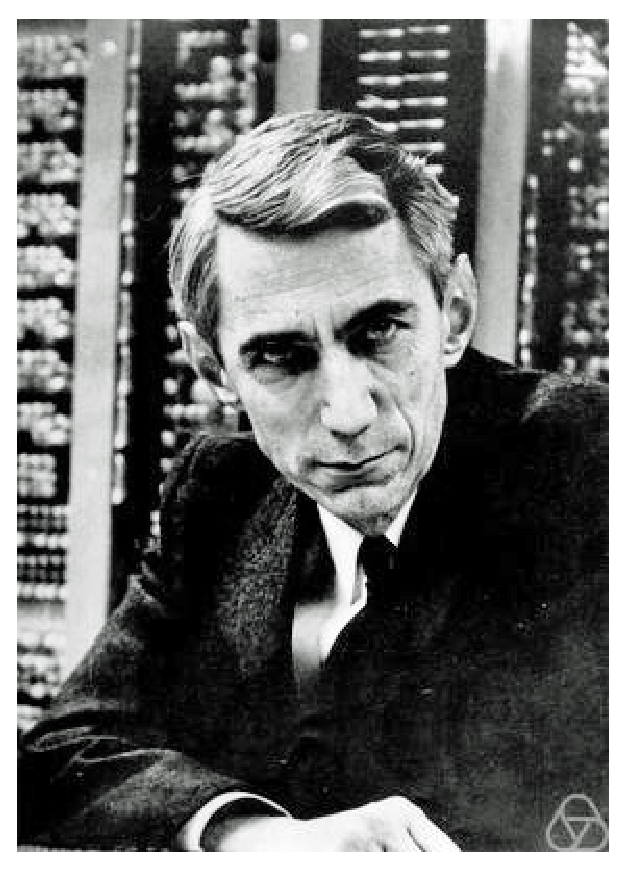
\includegraphics[width=0.8\linewidth]{ClaudeShannon.eps}
    \caption*{\textbf{Claude Shannon} (1916-2001), ingénieur et 
              mathématicien américain. 
              Père fondateur de la théorie de l'information.}
\end{marginfigure}
%-------------------------------------------------------------------------------
%-------------------------------------------------------------------------------
\begin{marginfigure}
    \centering
    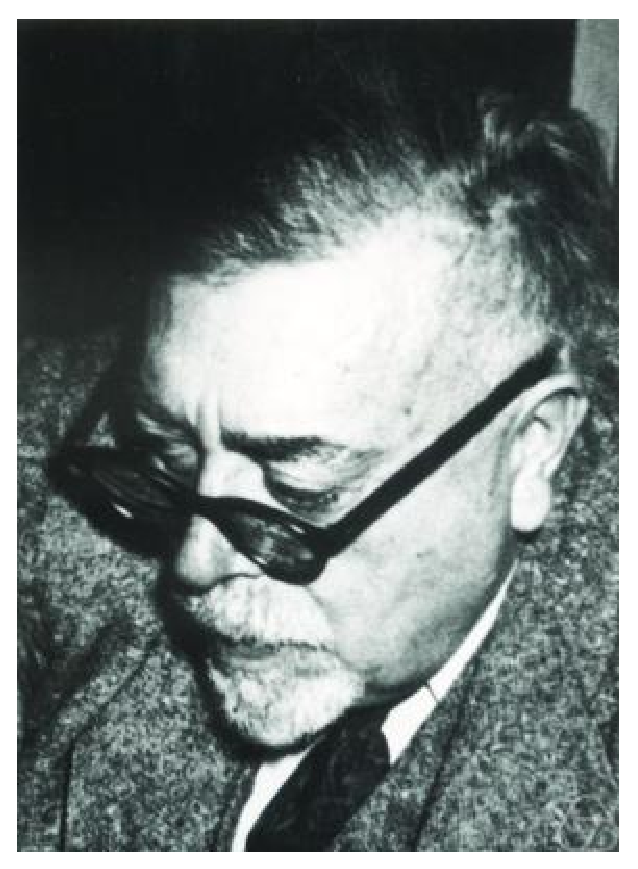
\includegraphics[width=0.8\linewidth]{NorbertWiener.eps}
    \caption*{\textbf{Norbert Wiener} (1894-1964), mathématicien 
              américain. Père fondateur de la cybernétique}
\end{marginfigure}
%-------------------------------------------------------------------------------
%-------------------------------------------------------------------------------
\begin{marginfigure}
    \centering
    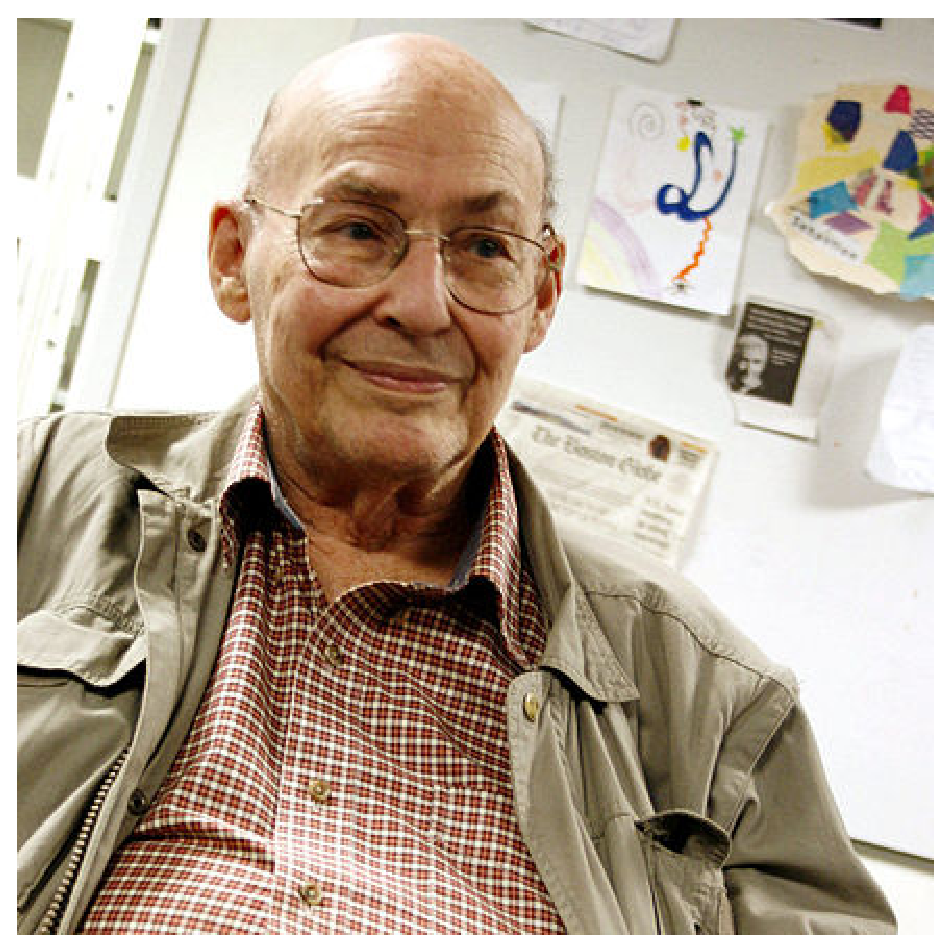
\includegraphics[width=0.8\linewidth]{MarvinMinsky.eps}
    \caption*{\textbf{Marvin Minsky} (1916-2001), mathématicien américain. 
              Auteur de l'expression \og intelligence artificielle\fg}
\end{marginfigure}
%-------------------------------------------------------------------------------

Au niveau structurel, \textbf{un système est un ensemble 
d'éléments constitutifs ayant des relations entre eux et présentant  
une frontière avec son environnement}. Cette définition est parfaitement
représenté par le schéma de la~\cref{fig-systeme}.
Au niveau fonctionnel, \textbf{un système modifie des flux dynamiques 
de matière, d'énergie et d'informations provenant 
de son environnement.}
\index{Système!monovariable}
\index{Système!multivariable}
C'est essentiellement cette dernière définition qui nous sera la plus utile.
Un système sera alors considéré comme une \og boîte\fg traitant une 
ou plusieurs entrées et élaborant une ou plusieurs sorties 
(c.f~\Cref{fig-systeme}). On distinguera les systèmes à 
une entrée et une sortie, dit \textbf{monovariable}\footnote{ou \gls{siso} 
en anglais} des systèmes  a plusieurs entrées et plusieurs sorties, dit 
\textbf{multivariable}\footnote{ou \gls{mimo} en anglais}.

\textbf{L'objectif de ce cours est de permettre la modélisation, 
l'identification et la caractérisation des systèmes monovariables.} 
\`A noter que cet objectif atteint, il nous sera possible de réprésenter 
les systèmes comme des \og boîtes noires\fg pour lesquelles la structure 
interne est inaccessible\footnote{\og Ce qui - en dernière analyse - justifie 
l'attitude ludique, c'est que le seul moyen concevable de dévoiler une 
boîte noire, c'est de jouer avec.\fg (René Thom)}. Une approche basée 
sur la représentation des états internes au système sera 
introduite au dernier chapitre de ce travail~\cref{chap-repreEtat}. 

Pour résumer, nous traiterons dans ce document 
des systèmes monovariables que nous représenterons simplement 
de la façon suivante :
%-------------------------------------------------------------------------------
\begin{center}
    \tikzsetnextfilename{sb_bloc-chap_slci-ext}
    \begin{tikzpicture}
    \sbEntree{E1}
    \sbBloc[3]{B1}{\Large$\Sigma$}{E1}
    \sbRelier[$e(t)$]{E1}{B1}
    \sbSortie[3]{S1}{B1}
    \sbRelier[$s(t)$]{B1}{S1}
\end{tikzpicture}

\end{center}
%-------------------------------------------------------------------------------
où $e(t)$ et $s(t)$ sont respectivement les signaux d'entrée et de sortie 
dépendants du temps et $\Sigma$ est le système traitant l'entrée $e(t)$ et 
élaborant la sortie $s(t)$ délimité par un bloc. 
Cette représentation, dite en \textbf{bloc} ou 
\textbf{schema-bloc}, sera généralisée au~\cref{chap-schemabloc}.
\clearpage
\restoregeometry
\captionsetup{width=0.9\linewidth,labelfont=bf}
%%%%%%%%%%%%%%%%%%%%%%%%%%%%%%%%%%%%%%%%%%%%%%%%%%%%%%%%%%%%%%%%%%%%%%%%%%%%%%%%
%%%%%%%%%%%%%%%%%%%%%%%%%%%%%%%%%%%%%%%%%%%%%%%%%%%%%%%%%%%%%%%%%%%%%%%%%%%%%%%%
\subsection{Propriétés des SLCI}
%%%%%%%%%%%%%%%%%%%%%%%%%%%%%%%%%%%%%%%%%%%%%%%%%%%%%%%%%%%%%%%%%%%%%%%%%%%%%%%%
%%%%%%%%%%%%%%%%%%%%%%%%%%%%%%%%%%%%%%%%%%%%%%%%%%%%%%%%%%%%%%%%%%%%%%%%%%%%%%%%
Les systèmes qui vont nous intéresser dans ce document sont les systèmes
\textbf{linéaires, continus et invariants}. Nous allons ici donner une 
définition de chacune de ces propriétés ainsi que des propriétés secondaires 
que nous rencontrerons au cours de notre étude.
%%%%%%%%%%%%%%%%%%%%%%%%%%%%%%%%%%%%%%%%%%%%%%%%%%%%%%%%%%%%%%%%%%%%%%%%%%%%%%%%
\paragraph{Système linéaire}
%%%%%%%%%%%%%%%%%%%%%%%%%%%%%%%%%%%%%%%%%%%%%%%%%%%%%%%%%%%%%%%%%%%%%%%%%%%%%%%%
\index{Système!linéaire}
Un système est dit linéaire si il respecte les deux principes suivants:
%-------------------------------------------------------------------------------
\begin{itemize}
    \item \emph{Principe de proportionnalité :}
        \textbf{Si $s(t)$ est la réponse à une entrée $e(t)$, alors 
        pour une entrée $\alpha e(t)$ la réponse est $\alpha s(t)$.}
        
        On exprime, schématiquement, ce principe de la façon suivante pour 
        un système linéaire $\Sigma$:
%-------------------------------------------------------------------------------
        \begin{center}
            \tikzsetnextfilename{principe_linearite-chap_slci-ext}
            \input{tikz/principe_linearite-chap_slci.tex}
        \end{center}
%-------------------------------------------------------------------------------
    \item \emph{Principe de superposition :}
        \textbf{Si l'entrée du système se décompose en une somme 
        de plusieurs entrées alors la sortie du système sera la somme des 
        sorties correspondant à chaque entrée séparée.}

        Une nouvelle fois, il est possible d'exprimer ce principe de la façon 
        suivante pour un système linéaire $\Sigma$:
%-------------------------------------------------------------------------------
        \begin{center}
            \tikzsetnextfilename{principe_superposition_1-chap_slci-ext}
            \begin{tikzpicture}
    \begin{scope}[local bounding box=scope1]
        \sbEntree{E1}
        \sbBloc[3]{B1}{\Large$\Sigma$}{E1}
        \node[] at ($(E1.west)+(-0.5,-0.9cm)$) {Si};
        \sbRelier[$e_1(t)$]{E1}{B1}
        \sbSortie[3]{S1}{B1}
        \sbRelier[$s_1(t)$]{B1}{S1}
    \end{scope}
    \begin{scope}[local bounding box=scope2,shift={($(E1)+(0,-2cm)$)}]
        \sbEntree{E2}
        \sbBloc[3]{B2}{\Large$\Sigma$}{E2}
        \sbRelier[$e_2(t)$]{E2}{B2}
        \sbSortie[3]{S2}{B2}
        \sbRelier[$s_2(t)$]{B2}{S2}
    \end{scope}
    \draw[thick,decorate,decoration={brace}] 
    ($(scope2.south west)+(0,0)$) -- ($(scope1.north west)+(0.8,0)$) ;
    \begin{scope}[shift={($(scope1.east)+(1.5,-0.7)$)}]
        \sbEntree{E3}
        \node[] at ($(E3.west)+(-0.5,0)$) {alors};
        \sbBloc[6]{B3}{\Large$\Sigma$}{E3}
        \sbRelier[$e_1(t)+e_2(t)$]{E3}{B3}
        \sbSortie[6]{S3}{B3}
        \sbRelier[$s_1(t)+s_2(t)$]{B3}{S3}
    \end{scope}
\end{tikzpicture}

        \end{center}
%-------------------------------------------------------------------------------
        Notons que ceci reste vrai pour une combinaison linéaire des entrées :
%-------------------------------------------------------------------------------
        \begin{center}
            \tikzsetnextfilename{principe_superposition_2-chap_slci-ext}
            \input{tikz/principe_superposition_2-chap_slci.tex}
        \end{center}
%-------------------------------------------------------------------------------
        avec $\alpha\ \text{et}\ \beta\in\mathbb{R}$, ou un nombre quelconques 
        d'entrées.
        %\[ 
        % s(t)=\sum_{k}^n \alpha_ks_k(t)
        %\]
\end{itemize}
%-------------------------------------------------------------------------------
%%%%%%%%%%%%%%%%%%%%%%%%%%%%%%%%%%%%%%%%%%%%%%%%%%%%%%%%%%%%%%%%%%%%%%%%%%%%%%%%
\paragraph{Système à temps continu}
%%%%%%%%%%%%%%%%%%%%%%%%%%%%%%%%%%%%%%%%%%%%%%%%%%%%%%%%%%%%%%%%%%%%%%%%%%%%%%%%
\index{Système!à temps continu}
\textbf{Un système à temps continu met en oeuvre des signaux 
à temps continus}. Comme nous le verrons, ces signaux seront
modélisés par des fonctions d'une variable continue $t$ de temps.
%%%%%%%%%%%%%%%%%%%%%%%%%%%%%%%%%%%%%%%%%%%%%%%%%%%%%%%%%%%%%%%%%%%%%%%%%%%%%%%%
\paragraph{Système invariant}
%%%%%%%%%%%%%%%%%%%%%%%%%%%%%%%%%%%%%%%%%%%%%%%%%%%%%%%%%%%%%%%%%%%%%%%%%%%%%%%%
\index{Système!invariant}
\textbf{Un système est dit invariant si la sortie ne dépend pas 
explicitement du temps autrement que par l'intermédiaire de l'entrée.}

On représente, schématiquement, un système invariant $\Sigma$, à 
l'aide d'un schéma-bloc ci-dessous 
(avec $\tau$ un temps quelconque.): 
%-------------------------------------------------------------------------------
\begin{center}
    \tikzsetnextfilename{sb_bloc_e3-chap_slci-ext}
    \input{tikz/principe_invariance-chap_slci.tex}
\end{center}
%-------------------------------------------------------------------------------
%%%%%%%%%%%%%%%%%%%%%%%%%%%%%%%%%%%%%%%%%%%%%%%%%%%%%%%%%%%%%%%%%%%%%%%%%%%%%%%%
\paragraph{Système causal}
%%%%%%%%%%%%%%%%%%%%%%%%%%%%%%%%%%%%%%%%%%%%%%%%%%%%%%%%%%%%%%%%%%%%%%%%%%%%%%%%
\index{Système!causal}
%-------------------------------------------------------------------------------
\begin{itemize}
    \item \emph{Principe de causalité :}
        C'est un principe fort de la physique :
        \textbf{\og L'éffet ne précèdant pas sa cause\fg} alors 
        \textbf{\og La réponse du système ne précède pas son excitation\fg}.
        Formellememnt, un système est dit causal si 
        \[ e(t)=0\quad\forall t\le t_0 \Rightarrow s(t)=0\quad\forall t\le t_0\]
\end{itemize}
%-------------------------------------------------------------------------------
%%%%%%%%%%%%%%%%%%%%%%%%%%%%%%%%%%%%%%%%%%%%%%%%%%%%%%%%%%%%%%%%%%%%%%%%%%%%%%%%
\paragraph{Système stable}
%%%%%%%%%%%%%%%%%%%%%%%%%%%%%%%%%%%%%%%%%%%%%%%%%%%%%%%%%%%%%%%%%%%%%%%%%%%%%%%%
\index{Système!stable}
Il existe deux définitions équivalentes de la stabilité pour 
un système linéaire:
%-------------------------------------------------------------------------------
\begin{itemize}
    \item \textbf{Un système est dit stable si à une entrée bornée le système 
        produit une sortie bornée} on parle de stabilité du type \gls{ebsb}.
          \footnote{Chez nos collègues anglo-saxons, 
          on rencontre la notion de BIBO (\og bounded input bounded output\fg)}
    \item \textbf{Un système est dit stable lorsque écarté de sa position 
           d'équilibre, il tend à y revenir}
\end{itemize}
%-------------------------------------------------------------------------------
Nous aurons l'occasion de préciser cette définition par des exemples plus 
concrets lorsque les outils de modélisation des systèmes et des signaux 
auront été introduits. Le \cref{chap-stab} est d'ailleurs totalement dédié 
à l'étude de cette propriété fondamentale.  
%%%%%%%%%%%%%%%%%%%%%%%%%%%%%%%%%%%%%%%%%%%%%%%%%%%%%%%%%%%%%%%%%%%%%%%%%%%%%%%%
%%%%%%%%%%%%%%%%%%%%%%%%%%%%%%%%%%%%%%%%%%%%%%%%%%%%%%%%%%%%%%%%%%%%%%%%%%%%%%%%
%%%%%%%%%%%%%%%%%%%%%%%%%%%%%%%%%%%%%%%%%%%%%%%%%%%%%%%%%%%%%%%%%%%%%%%%%%%%%%%%
\section{Modélisation d'un SLCI}
%%%%%%%%%%%%%%%%%%%%%%%%%%%%%%%%%%%%%%%%%%%%%%%%%%%%%%%%%%%%%%%%%%%%%%%%%%%%%%%%
%%%%%%%%%%%%%%%%%%%%%%%%%%%%%%%%%%%%%%%%%%%%%%%%%%%%%%%%%%%%%%%%%%%%%%%%%%%%%%%%
%%%%%%%%%%%%%%%%%%%%%%%%%%%%%%%%%%%%%%%%%%%%%%%%%%%%%%%%%%%%%%%%%%%%%%%%%%%%%%%%
%%%%%%%%%%%%%%%%%%%%%%%%%%%%%%%%%%%%%%%%%%%%%%%%%%%%%%%%%%%%%%%%%%%%%%%%%%%%%%%%
%%%%%%%%%%%%%%%%%%%%%%%%%%%%%%%%%%%%%%%%%%%%%%%%%%%%%%%%%%%%%%%%%%%%%%%%%%%%%%%%
\subsection{\'Equation différentielle à coefficients constants}
%%%%%%%%%%%%%%%%%%%%%%%%%%%%%%%%%%%%%%%%%%%%%%%%%%%%%%%%%%%%%%%%%%%%%%%%%%%%%%%%
%%%%%%%%%%%%%%%%%%%%%%%%%%%%%%%%%%%%%%%%%%%%%%%%%%%%%%%%%%%%%%%%%%%%%%%%%%%%%%%%
Les systèmes possédant les propriétés précédentes sont dit \textbf{linéaires 
continus et invariants} ou \gls{slci}. Ceux-ci seront modélisés et régis 
par une équation différentielle à coefficients 
constants qui s'écrit dans le cas générale :
%-------------------------------------------------------------------------------
\begin{bequation}[ams align]
\sum_{i=c}^{n}a_i\devi{s(t)}{i}=\sum_{i=0}^{m}b_i\devi{e(t)}{i}
\label{eq-difflci}
\end{bequation}
%-------------------------------------------------------------------------------
avec $n,m,c,\in\mathbb{N}$, $s(t)$ le signal de sortie, $e(t)$ le signal 
d'entrée et $a_i,b_i\in\mathbb{R}$ sont des coefficients constants. 

Le degré de dérivation de la sortie $n$ le plus grand est appelé \textbf{ordre}.
On parlera alors de \textbf{l'ordre du système} $n$. Le paramètre $c$ qui 
correspond au degré de dérivation le plus petit de la sortie est appelé la
\textbf{classe du système}.
%%%%%%%%%%%%%%%%%%%%%%%%%%%%%%%%%%%%%%%%%%%%%%%%%%%%%%%%%%%%%%%%%%%%%%%%%%%%%%%%
\paragraph{Exemples}
%%%%%%%%%%%%%%%%%%%%%%%%%%%%%%%%%%%%%%%%%%%%%%%%%%%%%%%%%%%%%%%%%%%%%%%%%%%%%%%%
Pour un système d'ordre $n=2$, de classe 0 et avec $m=0$, 
son équation différentielle sera alors de la forme :
\[
    a_2\devi{s(t)}{2}+a_1\devi{s(t)}{}+a_0 s(t)=b_0e(t)
\]
%ou encore pour un système d'ordre $n=3$, de classe 
%$c=1$ et avec $m=1$, l'équation différentielle sera de la forme :
%\[
%    a_3\devi{s(t)}{3}+a_2\devi{s(t)}{2}+a_1\devi{s(t)}{}
%    =b_0e(t)+b_1\devi{e(t)}{}
%\]
\input{re/newgeometry}
\captionsetup{width=0.9\linewidth,labelfont=bf}
%%%%%%%%%%%%%%%%%%%%%%%%%%%%%%%%%%%%%%%%%%%%%%%%%%%%%%%%%%%%%%%%%%%%%%%%%%%%%%%%
%%%%%%%%%%%%%%%%%%%%%%%%%%%%%%%%%%%%%%%%%%%%%%%%%%%%%%%%%%%%%%%%%%%%%%%%%%%%%%%%
\subsection{Exemples de mises en équation}
%%%%%%%%%%%%%%%%%%%%%%%%%%%%%%%%%%%%%%%%%%%%%%%%%%%%%%%%%%%%%%%%%%%%%%%%%%%%%%%%
%%%%%%%%%%%%%%%%%%%%%%%%%%%%%%%%%%%%%%%%%%%%%%%%%%%%%%%%%%%%%%%%%%%%%%%%%%%%%%%%
Pour un problème donné, ces équations différentielles proviennent 
directement de la modélisation de la physique (qu'il soit mécanique, 
électronique, thermique \ldots).
Par exemple, dans le cas d'un problème de mécanique, 
c'est la relation fondamentale de la dynamique qui est 
la source importante d'équations différentielles (appelées équations 
du mouvement).
En électronique, ce sont, par exemple, les lois des noeuds et mailles (ou 
lois de Kirchhoff) qui permettront d'écrire ces équations différentielles. 
%%%%%%%%%%%%%%%%%%%%%%%%%%%%%%%%%%%%%%%%%%%%%%%%%%%%%%%%%%%%%%%%%%%%%%%%%%%%%%%%
\paragraph{Décharge d'un condensateur\label{para-decharge}}
%%%%%%%%%%%%%%%%%%%%%%%%%%%%%%%%%%%%%%%%%%%%%%%%%%%%%%%%%%%%%%%%%%%%%%%%%%%%%%%%
Considérons le circuit ouvert ci-contre, initialement chargé, constitué 
d'un condensateur de capacité électrique $C$ et d'une résistance de valeur $R$. 
À la fermeture de l'interrupteur, à $t=0$, un courant $i(t)$ parcourt 
le circuit. On observe alors la décharge du condensateur à travers 
une resistance $R$. 

On souhaite suivre la quantité de charge $q(t)$ aux bornes du condensateur au 
cours du temps.
%-------------------------------------------------------------------------------
\begin{marginfigure}[-8em]   
    \centering
    \tikzsetnextfilename{decharge_condensateur-chap_slci-ext}
    %               K           
%     A ------B    C---------D
%     |                      |
%     |                      |
% C1--E--C2                --J-R2 
%                          |   |
% C3--F--C4               R1-I--
%     |                      |
%     |                      |
%     G----------------------H
%
%
\begin{tikzpicture}

    \pgfmathsetmacro{\pC}{0.75}   % distance de C(1,2,3,4) en x relativement E/F
    \pgfmathsetmacro{\eC}{0.5}    % ecartement du condensateur E-F
    \pgfmathsetmacro{\lR}{1.25}   % longueur de la resistance
    \pgfmathsetmacro{\pR}{0.25}   % position de R1 / I
    \pgfmathsetmacro{\eR}{2*\pR}
    \pgfmathsetmacro{\ab}{1.5}
    \pgfmathsetmacro{\cb}{1.0}
    \pgfmathsetmacro{\gh}{2*\ab+\cb}
    \pgfmathsetmacro{\fg}{1}
    \pgfmathsetmacro{\tmpu}{0.5*\eC}
    \pgfmathsetmacro{\tmpd}{-0.5*\lR}
    \pgfmathsetmacro{\dj}{\fg+\tmpu+\tmpd}

    \coordinate (A)  at (0,0);
    \coordinate (B)  at ($(A)+(\ab,0)$);
    \coordinate (C)  at ($(B)+(\cb,0)$);
    \coordinate (D)  at ($(C)+(\ab,0)$);
    \coordinate (E)  at ($(A)+(0,-\fg)$);
    \coordinate (F)  at ($(E)+(0,-\eC)$);
    \coordinate (C1) at ($(E)+(-\pC,0)$);
    \coordinate (C2) at ($(E)+(\pC,0)$);
    \coordinate (C3) at ($(F)+(-\pC,0)$);
    \coordinate (C4) at ($(F)+(\pC,0)$);
    \coordinate (G)  at ($(F)+(0,-\fg)$);
    \coordinate (H)  at ($(G)+(\gh,0)$);
    \coordinate (I)  at ($(H)+(0,\dj)$);
    \coordinate (J)  at ($(I)+(0,\lR)$);
    \coordinate (K)  at ($(C)+(-0.75,0.5)$);
    \coordinate (R1) at ($(I)+(-\pR,0)$);
    \coordinate (R2) at ($(R1)+(\eR,\lR)$);

    %\node[circle,fill=white,draw=black,ultra thick] at (B) {};
    \draw[thick] (A)  -- (B);
    \draw[thick] (C)  -- (D);
    \draw[thick] (A)  -- (E);
    \draw[very thick,col1] (C1) -- (C2) 
    node[col1,xshift=1em,yshift=-0.5em] {$C$};
    \draw[very thick,col1] (C3) -- (C4);
    \draw[thick] (F)  -- (G);
    \draw[thick] (G)  -- (H);
    \draw[thick] (I)  -- (H);
    \draw[thick] (J)  -- (D);
    \draw[thick] (K)  -- (C);
    \draw[very thick,col4] (R1) rectangle (R2) 
    node[yshift=-1.5em,xshift=0.75em] {$R$};
    \draw[draw=black,fill=white] (B) circle (2pt);
    \draw[draw=black,fill=white] (C) circle (2pt);
\end{tikzpicture}

    \caption{Circuit RC ouvert.\label{fig-decharge_condensateur}}
\end{marginfigure}
%-------------------------------------------------------------------------------
La somme des tensions aux bornes du condensateur et de la résistance 
étant nulle, on a :
%-------------------------------------------------------------------------------
\begin{align*}
    R\devi{q(t)}{}+\dfrac{1}{C}q(t)=0 
\end{align*}
%-------------------------------------------------------------------------------
Comme précédemment, on identifie formellemet cette équation différentielle 
à la forme générale de l'\cref{eq-difflci} avec $s(t)=q(t)$, $e(t)=0$, 
$n=$1, $m=0$, $a_1=R$, $a_0=\dfrac{1}{C}$.

Nous laissons au lecteur la résolution de cette équation différentielle 
par une approche direct classique. Sa résolution utilisant la transformée 
de Laplace, est présenté en exercice à la fin de ce chapitre.
%Nous la rencontrerons à nouveau au~\cref{chap-model}, après avoir 
%présenté la méthode générale pour la résolution de ce type d'équation.
%%%%%%%%%%%%%%%%%%%%%%%%%%%%%%%%%%%%%%%%%%%%%%%%%%%%%%%%%%%%%%%%%%%%%%%%%%%%%%%%
\paragraph{Système masse-ressort\label{para-masse_ressort}}
%%%%%%%%%%%%%%%%%%%%%%%%%%%%%%%%%%%%%%%%%%%%%%%%%%%%%%%%%%%%%%%%%%%%%%%%%%%%%%%%
On considère un système mécanique constitué d'une masse $m$ en translation 
couplée avec un ressort de constante
de raideur $k$ et un amortisseur de coefficient de frottement 
visqueux $b$ (c.a.d que la force est 
proportionnelle à la vitesse). 
La masse est soumise à une force $\vect{f}=f(t)\zz{}$.
%-------------------------------------------------------------------------------
\begin{marginfigure}[-8em]
    \centering
    \tikzsetnextfilename{masse_ressort-chap_slci-ext}
    \input{tikz/masse_ressort-chap_slci.tex}
    \caption{(gauche) Système masse-ressort. (droite) Schéma-bloc de ce même 
    système.
    \label{fig-masse-ressort}}
\end{marginfigure}
%-------------------------------------------------------------------------------
En appliquant le principe fondamentale de la dynamique en projection 
sur le vecteur $\zz{}$, on obtient l'équation du mouvement suivante :
\[
m\devi{z(t)}{2}+b\devi{z(t)}{}+kz(t)=f(t)
\]
\newpage
\restoregeometry
\captionsetup{width=0.9\linewidth,labelfont=bf}
La résolution de cette équation du mouvement permet de connaitre la position 
de la masse à chaque instant connaissant la force exterieur 
appliquée $f(t)$. Le système masse-ressort peut être assimilé à un~\gls{slci} 
dont l'entrée $e(t)$ est la force $f(t)$ et la sortie $s(t)$ est la 
position $z(t)$ de la masse (c.f le schéma-bloc de la \cref{fig-masse-ressort})

On identifie simplement, cette équation différentielle à la forme générale 
de l'\cref{eq-difflci} pour $s(t)=z(t)$, $e(t)=f(t)$, 
$n=$2, $m=0$, $a_2=m$, $a_1=b$, $a_0=k_r$ et $b_0=$1.
La résolution complète sera donnée en exercice à la fin de ce chapitre.
%%%%%%%%%%%%%%%%%%%%%%%%%%%%%%%%%%%%%%%%%%%%%%%%%%%%%%%%%%%%%%%%%%%%%%%%%%%%%%%%
%%%%%%%%%%%%%%%%%%%%%%%%%%%%%%%%%%%%%%%%%%%%%%%%%%%%%%%%%%%%%%%%%%%%%%%%%%%%%%%%
%%%%%%%%%%%%%%%%%%%%%%%%%%%%%%%%%%%%%%%%%%%%%%%%%%%%%%%%%%%%%%%%%%%%%%%%%%%%%%%%
\section{Modélisation d'un signal}
%%%%%%%%%%%%%%%%%%%%%%%%%%%%%%%%%%%%%%%%%%%%%%%%%%%%%%%%%%%%%%%%%%%%%%%%%%%%%%%%
%%%%%%%%%%%%%%%%%%%%%%%%%%%%%%%%%%%%%%%%%%%%%%%%%%%%%%%%%%%%%%%%%%%%%%%%%%%%%%%%
%%%%%%%%%%%%%%%%%%%%%%%%%%%%%%%%%%%%%%%%%%%%%%%%%%%%%%%%%%%%%%%%%%%%%%%%%%%%%%%%
\textbf{Un signal est une variation d'une grandeur qui porte l'information 
de la sollicitation ou de la réponse d'un système.}

Les signaux continus sont modélisés mathématiquement par des fonctions 
continues du temps. Formellement, par une fonction $s$ telle que :
%-------------------------------------------------------------------------------
\begin{align*}
s : \mathbb{R}&\rightarrow\mathbb{R} \\  
t&\rightarrow s(t) 
\end{align*}    
%-------------------------------------------------------------------------------
Il existe cependant d'autres types de signaux qui sont très souvent confondus 
à tort:
%-------------------------------------------------------------------------------
\begin{itemize}
    \item un signal \emph{quantifié} est un signal continu 
          dont la valeur ne peut prendre que des valeurs discrètes. 
    \item un signal \emph{discret} est un signal à temps discret.
    \item un signal \emph{numérique} est un signal discret et quantifié.   
\end{itemize}
%-------------------------------------------------------------------------------
\textbf{Dans le reste de ce document, nous ne traiterons que
du cas de signaux en temps continu}. Les signaux en temps discret
sont généralement abordées lors d'un cours 
avancé d'automatique en cycle ingénieur.
%\newpage
%%%%%%%%%%%%%%%%%%%%%%%%%%%%%%%%%%%%%%%%%%%%%%%%%%%%%%%%%%%%%%%%%%%%%%%%%%%%%%%%
%%%%%%%%%%%%%%%%%%%%%%%%%%%%%%%%%%%%%%%%%%%%%%%%%%%%%%%%%%%%%%%%%%%%%%%%%%%%%%%%
\subsection{Propriétés des signaux continus}
%%%%%%%%%%%%%%%%%%%%%%%%%%%%%%%%%%%%%%%%%%%%%%%%%%%%%%%%%%%%%%%%%%%%%%%%%%%%%%%%
%%%%%%%%%%%%%%%%%%%%%%%%%%%%%%%%%%%%%%%%%%%%%%%%%%%%%%%%%%%%%%%%%%%%%%%%%%%%%%%%
%%%%%%%%%%%%%%%%%%%%%%%%%%%%%%%%%%%%%%%%%%%%%%%%%%%%%%%%%%%%%%%%%%%%%%%%%%%%%%%%
\paragraph{Causal}
%%%%%%%%%%%%%%%%%%%%%%%%%%%%%%%%%%%%%%%%%%%%%%%%%%%%%%%%%%%%%%%%%%%%%%%%%%%%%%%%
\index{Signal!causal}
Un signal modélisé par la fonction $s(t)$ est dit \textbf{causal}
si ce signal est nul pour tout $t<0$. Pour un signal en entrée, le temps 
$t=0$ permet de définir une origine des temps.
%-------------------------------------------------------------------------------
\begin{figure}[!h]
    \centering
    \tikzsetnextfilename{causal-chap_slci-ext}
    \input{tikz/causal-chap_slci.tex}
\end{figure}
%-------------------------------------------------------------------------------
%%%%%%%%%%%%%%%%%%%%%%%%%%%%%%%%%%%%%%%%%%%%%%%%%%%%%%%%%%%%%%%%%%%%%%%%%%%%%%%%
\paragraph{Retardé}
%%%%%%%%%%%%%%%%%%%%%%%%%%%%%%%%%%%%%%%%%%%%%%%%%%%%%%%%%%%%%%%%%%%%%%%%%%%%%%%%
\index{Signal!retardé}
Un signal $s(t-\tau)$ est dit \textbf{retardé} d'un temps $\tau$ 
par rapport à $s(t)$, si on lui a fait subir un changement
d'origine des temps par rapport au signal $s(t)$.
%-------------------------------------------------------------------------------
\begin{center}
    \tikzsetnextfilename{retarde-chap_slci-ext}
    \input{tikz/retarde-chap_slci.tex}
\end{center}
%-------------------------------------------------------------------------------
%%%%%%%%%%%%%%%%%%%%%%%%%%%%%%%%%%%%%%%%%%%%%%%%%%%%%%%%%%%%%%%%%%%%%%%%%%%%%%%%
\paragraph{Périodique}
%%%%%%%%%%%%%%%%%%%%%%%%%%%%%%%%%%%%%%%%%%%%%%%%%%%%%%%%%%%%%%%%%%%%%%%%%%%%%%%%
\index{Signal!périodique}
Un signal est dit \textbf{périodique} s'il se reproduit identique à lui
même au bout d'un même intervalle de temps ou periode $T$. On définit alors 
sa fréquence $f=1/T$ qui est l'inverse de la période $T$ ou la pulsation 
$\omega$ définie par rapport au cercle unité $\omega=2\pi f$.
%-------------------------------------------------------------------------------
\begin{figure}[!htb]
    \centering
    \tikzsetnextfilename{periodique-chap_slci-ext}
    \begin{tikzpicture}
    \begin{axis}
    [	ticks=none,
        axis line style = thick,
        height=5cm,
        width=9cm,
        axis x line=center,
        axis y line=center,
        xmin=-2,
        xmax=16,
        ymin=-2.0,
        ymax=2.0,
        xlabel={$t$},
        ylabel={$s(t)$},
        xlabel style={below right},
        ylabel style={above left},
        clip bounding box=upper bound,
        enlargelimits=false
    ]
    \addplot[very thick,col1,domain=-2:0, samples=101] {0};
    \addplot[very thick,col1,domain=0:2, samples=101]  {0.5*x};
    \addplot[very thick,col1,domain=2:6, samples=101]  {-0.5*x+2};
    \addplot[very thick,col1,domain=6:10, samples=101] {0.5*x-4};
    \addplot[very thick,col1,domain=10:14, samples=101]{-0.5*x+6};
    \draw[col1] (axis cs:2,1) -- (axis cs:2,1.25);
    \draw[col1] (axis cs:10,1) -- (axis cs:10,1.25);
    \draw[col1,ultra thick, latex-latex] (axis cs:2,1.25) -- 
    node[above,yshift=+0.2em]{$T$} (axis cs:10,1.25);
    \end{axis}
\end{tikzpicture}

\end{figure}
%-------------------------------------------------------------------------------
Le signal complet peut être totalement d'écrit en considérant un motif de base 
$s_0(t)$ tel que
%-------------------------------------------------------------------------------
\begin{align*}
    s_0(t) =
    \begin{dcases}
        s(t)&\quad\text{pour}\quad 0\le t\le T   \\
        0&\quad\text{pour}\quad t>T
    \end{dcases}
\end{align*}
%-------------------------------------------------------------------------------
Le signal $s(t)$ est alors la somme (série) du motif retardé de $nT$ 
avec $n\in\mathbb{N}$ tel que :
\[
s(t)=\sum_0^\infty s_0(t-nT)
\]
L'analyse de Fourier est un outil fondamental pour l'étude 
de ces signaux périodiques. Elle sort cependant légèrement du cadre de 
ce cours. (c.f~\Cref{annexe-seriefourier}).
%%%%%%%%%%%%%%%%%%%%%%%%%%%%%%%%%%%%%%%%%%%%%%%%%%%%%%%%%%%%%%%%%%%%%%%%%%%%%%%%
\paragraph{Stable}
%%%%%%%%%%%%%%%%%%%%%%%%%%%%%%%%%%%%%%%%%%%%%%%%%%%%%%%%%%%%%%%%%%%%%%%%%%%%%%%%
\index{Signal!stable}
En se basant sur la définition donnée d'un système stable.
Nous ne limiterons à dire qu'un signal stable est un signal 
borné. Les signaux usuels en entrée de nos systèmes sont bornés 
et stables.

La~\cref{fig-stabilite_signaux} présente un exemple qualitatif de réponses 
stables et instables pour deux sollicitations bornées (respectivement une 
sollicitation constante et une sollicitation oscillante).
%-------------------------------------------------------------------------------
\begin{figure}[!ht]
    \centering
    \tikzsetnextfilename{entree_echelon-chap_slci_ext}
    \input{tikz/entree_echelon-chap_slci.tex}
    \tikzsetnextfilename{stable_echelon-chap_slci_ext}
    \input{tikz/stable_echelon-chap_slci.tex}
    \tikzsetnextfilename{instable_echelon-chap_slci_ext}
    \begin{tikzpicture}
    \begin{axis}
    [	ticks=none,
        axis line style = thick,
        height=5cm,
        width=5cm,
        axis x line=center,
        axis y line=center,
        xmin=-2,
        xmax=10,
        ymin=-0.5,
        ymax=2.0,
        xlabel={$t$},
        ylabel={$s(t)$},
        xlabel style={below right},
        ylabel style={above left},
    ]
    \addplot[signalr,domain=-2:0]  {0};
    \addplot[signalr,domain=0:10] {0.05*x^2};
    \end{axis}
\end{tikzpicture}


    \tikzsetnextfilename{entree_harm-chap_slci_ext}
    \begin{tikzpicture}
    \begin{axis}
    [   ticks=none,
        axis line style = thick,
        height=5cm,
        width=5cm,
        axis x line=center,
        axis y line=center,
        xmin=-2,
        xmax=10,
        ymin=-2.0,
        ymax=2.0,
        xlabel={$t$},
        ylabel={$e(t)$},
        xlabel style={below right},
        ylabel style={above left},
    ]
    \addplot[signaln,domain=-2:0]  {0};
    \addplot[signaln,domain=0:9.5]  {sin(deg(2*x))};
    \end{axis}
\end{tikzpicture}

    \tikzsetnextfilename{stable_harm-chap_slci_ext}
    \input{tikz/stable_harm-chap_slci.tex}
    \tikzsetnextfilename{instable_harm-chap_slci_ext}
    \begin{tikzpicture}%
    \begin{axis}
    [	ticks=none,
        axis line style = thick,
        height=5cm,
        width=5cm,
        axis x line=center,
        axis y line=center,
        xmin=-2,
        xmax=10,
        ymin=-5,
        ymax=5,
        xlabel={$t$},
        ylabel={$s(t)$},
        xlabel style={below right},
        ylabel style={above left},
    ]
    \addplot[signalr,domain=-2:0]  {0};
    \addplot[signalr,domain=0:9.5] {0.8*sin(3*deg(x))*exp(0.2*x)};
    \end{axis}
\end{tikzpicture}

    \caption{Trois exemples de réponses d'un SLCI à des sollicitations bornées :
            (en bleu)  réponses stables 
            (en rouge) réponses instables.\label{fig-stabilite_signaux}}
\end{figure}
%-------------------------------------------------------------------------------
\newpage
\input{re/newgeometry}
\captionsetup{width=0.9\linewidth,labelfont=bf}
%%%%%%%%%%%%%%%%%%%%%%%%%%%%%%%%%%%%%%%%%%%%%%%%%%%%%%%%%%%%%%%%%%%%%%%%%%%%%%%%
%%%%%%%%%%%%%%%%%%%%%%%%%%%%%%%%%%%%%%%%%%%%%%%%%%%%%%%%%%%%%%%%%%%%%%%%%%%%%%%%
\subsection{Signaux usuels rencontrés\ldots\label{sec-signaux_usuels}}
%%%%%%%%%%%%%%%%%%%%%%%%%%%%%%%%%%%%%%%%%%%%%%%%%%%%%%%%%%%%%%%%%%%%%%%%%%%%%%%%
%%%%%%%%%%%%%%%%%%%%%%%%%%%%%%%%%%%%%%%%%%%%%%%%%%%%%%%%%%%%%%%%%%%%%%%%%%%%%%%%
%Nous aurons l'occasion de rencontrer de nombreuses fois certains signaux.
Certains signaux sont des briques de base pour la construction de
signaux plus complexes. Il est alors essentiel de bien les caractériser.
Ici, nous distinguons les signaux généralement utilisés en 
entrée des signaux généralement rencontrées en sortie des \gls{slci}.
%%%%%%%%%%%%%%%%%%%%%%%%%%%%%%%%%%%%%%%%%%%%%%%%%%%%%%%%%%%%%%%%%%%%%%%%%%%%%%%%
\subsubsection{\ldots en entrée}
%%%%%%%%%%%%%%%%%%%%%%%%%%%%%%%%%%%%%%%%%%%%%%%%%%%%%%%%%%%%%%%%%%%%%%%%%%%%%%%%
%%%%%%%%%%%%%%%%%%%%%%%%%%%%%%%%%%%%%%%%%%%%%%%%%%%%%%%%%%%%%%%%%%%%%%%%%%%%%%%%
\paragraph{Impulsion de Dirac\index{Signaux usuels!Impulsion de Dirac}}
%%%%%%%%%%%%%%%%%%%%%%%%%%%%%%%%%%%%%%%%%%%%%%%%%%%%%%%%%%%%%%%%%%%%%%%%%%%%%%%%
L'impulsion de Dirac
$\delta(t)$ est une \og fonction\fg 
\footnote{Les guillemets sont essentiels pour ne pas se fâcher avec 
nos collègues mathématiciens. En effet, ce signal est un exemple classique de 
la théorie des distributions qui étend la notion de fonction.} telle que
%-------------------------------------------------------------------------------
\begin{marginfigure}
    \centering
    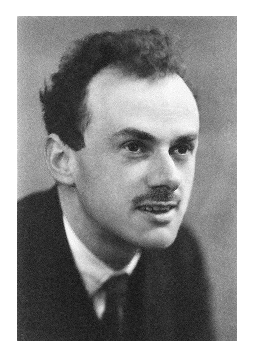
\includegraphics[width=0.9\linewidth]{PaulDirac.eps} 
    \caption{\index{Dirac, Paul}\textbf{Paul Dirac}, (1902-1984) 
              mathématicien et physicien britannique. Auteur de 
              contributions majeures en mécanique quantique. 
              \href{https://www.youtube.com/watch?v=H7mOU1Xu-yA}{Lien Youtube}
              } 
\end{marginfigure}
%-------------------------------------------------------------------------------
%-------------------------------------------------------------------------------
\begin{align*}
    \delta(t) : 
    \begin{dcases}
    	\int\limits_{-\infty}^{+\infty}	 \delta(t)\,\,\dd{t}&=1   \\
        \int\limits_{-\infty}^{+\infty}  \delta(t)f(t)\,\,\dd{t}&=f(0)	
    \end{dcases}
\end{align*}
%-------------------------------------------------------------------------------
Cette fonction est donc nulle partout sauf en $t=0$ où elle prend 
une valeur infinie. C'est pourquoi l'intégrale sur tous les nombres réels 
d'une impulsion de Dirac est normalisée à 1.
Graphiquement une impulsion de Dirac $\delta(t)$ est 
représentée par une flèche en $t=0$. La figure ci-dessous présente 
une impulsion de Dirac ainsi qu'une 
impulsion retardée de $\tau$ noté $\delta(t-\tau)$.
%-------------------------------------------------------------------------------
\begin{figure}[!h]
    \centering
    \tikzsetnextfilename{dirac-chap_slci-ext}
    \input{tikz/dirac-chap_slci.tex}
\end{figure}
%-------------------------------------------------------------------------------
L'impulsion de Dirac peut être expérimentalement approchée par un signal 
bref et de grande amplitude. La figure~\ref{fig-dirac2} représente un modèle 
approchée de l'impulsion de Dirac. Il est possible de montrer que cette fonction
$\delta_a(t)$ s'approche d'une impulsion de Dirac lorsque $a\to0$.
%-------------------------------------------------------------------------------
\begin{marginfigure}
    \centering
    \tikzsetnextfilename{dirac_reel-chap_slci-ext}
    \input{tikz/dirac_reel-chap_slci.tex}
    \caption{Représentation de l'impulsion de Dirac approchée. 
             Celle-ci tend vers l'impulsion de Dirac pour $a\to0$. 
             On remarquera que l'aire du rectangle est toujours égale à 1.
             \label{fig-dirac2}}
\end{marginfigure}
%-------------------------------------------------------------------------------

Nous rencontrerons quelque fois l'impulsion de Dirac sous sa forme généralisée, 
\[
e(t)=E_0\delta(t)
\]
où $e(t)$ est le signal d'entrée du système et $E_0$ la valeur de l'amplitude 
de l'impulsion de Dirac dont la dimension dépendra de la nature du 
problème considéré.
La réponse d'un système à une impulsion de Dirac est appelée 
\textbf{réponse impulsionnelle}.
Nous verrons par la suite qu'une telle sollicitation brève et de grande 
amplitude permet de parfaitement caractériser le système. La réponse 
impulsionnelle, qui en résulte, contient toute l'information sur le système 
linéaire qui l'a élaboré.
%%%%%%%%%%%%%%%%%%%%%%%%%%%%%%%%%%%%%%%%%%%%%%%%%%%%%%%%%%%%%%%%%%%%%%%%%%%%%%%%
\paragraph{\'Echelon-unité}
%%%%%%%%%%%%%%%%%%%%%%%%%%%%%%%%%%%%%%%%%%%%%%%%%%%%%%%%%%%%%%%%%%%%%%%%%%%%%%%%
\index{Signaux usuels!échelon unité}
L'échelon-unité est défini par la fonction, noté $u(t)$, telle que :
\[
    u(t)=
    \begin{cases} 
    0 \qquad \forall t<0    \\ 
    1 \qquad \forall t\geq 0 
    \end{cases}
\]
Cette fonction présente une marche\footnote{Nos 
collègues anglo-saxons l'appelle la \og\emph{step function}\fg} à $t=0$. 
Ci contre, nous la représentons avec la fonction retardée $u(t-\tau)$.
%-------------------------------------------------------------------------------
\begin{marginfigure}
    \centering
    \tikzsetnextfilename{echelon-chap_slci-ext}
    \input{tikz/echelon-chap_slci.tex}
    \caption{Représentation graphique de (haut) la fonction échelon-unité 
             et (bas) la fonction échelon-unité retardée de $\tau$
            \label{fig-echelon}}
\end{marginfigure}
%-------------------------------------------------------------------------------
En général, l'échelon-unité est utilisé en entrée de nos systèmes pour 
modéliser des états fermé/ouvert (\og on/off\fg) ou encore en régulation.
Nous la rencontrerons souvent sous sa forme généralisée, 
\[
    e(t)=E_0u(t)
\]
où $e(t)$ est le signal d'entrée du système et $E_0$ la valeur seuil 
de l'échelon dont la dimension dépend de la nature du problème considéré.

D'après les propriétés du signal échelon-unité et de la causalité, il 
est possible de rendre causale une fonction quelconque en la 
multipliant par un échélon-unité (c.f \ref{subsec:decomp_usuels}).

La réponse d'un système à un échelon est appelée 
\textbf{réponse indicielle}.

Remarquons que la fonction échelon-unité est l'intégrale 
de la distribution de Dirac,
%-------------------------------------------------------------------------------
\begin{equation}
    u(t)=\int\limits_{-\infty}^{t} \delta(\tau)\,\,\dd{\tau}
    \label{eq-echelon-dirac_relation}
\end{equation}
%-------------------------------------------------------------------------------
%-------------------------------------------------------------------------------
\begin{marginfigure}
    \centering
    \tikzsetnextfilename{rampe-chap_slci-ext}
    \begin{tikzpicture}
    \begin{axis}[
    name=ax2,
    ticks=none,
    axis line style = thick,
    height=4cm,
    width=5cm,
    axis x line=center,
    axis y line=center,
    xmin=-2,
    xmax=6,
    ymin=-1.5,
    ymax=6,
    xlabel={$t$},
    ylabel={$r(t)$},
    xlabel style={below right},
    ylabel style={above left},
    ]
    \addplot [ultra thick,col1,domain=-2:0, samples=101]{0};
    \addplot [ultra thick,col1,domain=0:15, samples=101]{x};
    \end{axis}
    \begin{axis}[
    at={(ax2.below south west)},
    anchor=north west,
    yshift=-0.9em,
    axis line style = thick,
    height=4cm,
    width=5cm,
    axis x line=center,
    axis y line=center,
    xmin=-2,
    xmax=8,
    ymin=-1.5,
    ymax=8,
    xlabel={$t$},
    ylabel={$r(t-\tau)$},
    xlabel style={below right},
    ylabel style={above left},
    xticklabels={$\tau$},
    xtick={2},
    ytick=\empty,
    ]
    \addplot [ultra thick,col1,domain=-2:2, samples=101]{0};
    \addplot [ultra thick,col1,domain=2:17, samples=101]{x-2};
    \end{axis}
\end{tikzpicture}

    \caption{Représentation graphique de (haut) la fonction rampe-unité et 
                                     (bas) la fonction rampe-unité retardée
                                     de $\tau$\label{fig-rampe}}
\end{marginfigure}
%-------------------------------------------------------------------------------
%%%%%%%%%%%%%%%%%%%%%%%%%%%%%%%%%%%%%%%%%%%%%%%%%%%%%%%%%%%%%%%%%%%%%%%%%%%%%%%%
\paragraph{Rampe-unité}
%%%%%%%%%%%%%%%%%%%%%%%%%%%%%%%%%%%%%%%%%%%%%%%%%%%%%%%%%%%%%%%%%%%%%%%%%%%%%%%%
\index{Signaux usuels!rampe unité}
Le signal rampe-unité\footnote{On retrouve parfois~\cite{sueurautomatique} 
le terme d'échelon vitesse pour désigner la fonction rampe} est
modélisé par la fonction $r(t)$ telle que :
\[
    r(t)=
    \begin{cases}
	0\,\,\,\,t<0 \\
	t\,\,\,\,t\geq0 
    \end{cases}
\]
ou autrement dit, en utilisant la propriété de causalité de l'échelon:
\[
    r(t)=t\cdot u(t)
\]
Remarquons que la fonction rampe est l'intégrale de l'échelon-unité, notamment 
%-------------------------------------------------------------------------------
\begin{equation}
    r(t)=\int\limits_{-\infty}^{t} u(\tau)\,\,\dd{\tau}
    \label{eq-rampe-echelon_relation}
\end{equation}
%-------------------------------------------------------------------------------
La réponse d'un système à une rampe ne possède pas de nom spécifique 
pour la distinguer des autres réponses. Nous parlerons donc simplement 
de \textbf{réponse à une rampe}. 
%%%%%%%%%%%%%%%%%%%%%%%%%%%%%%%%%%%%%%%%%%%%%%%%%%%%%%%%%%%%%%%%%%%%%%%%%%%%%%%%
\paragraph{Sinuso\"ide}
%%%%%%%%%%%%%%%%%%%%%%%%%%%%%%%%%%%%%%%%%%%%%%%%%%%%%%%%%%%%%%%%%%%%%%%%%%%%%%%%
\index{Signaux usuels!sinuso\"ide}
Le signal périodique sinuso\"idal $s(t)$ est la fonction telle que :
\[
    s(t)=A\sin{(\omega t +\phi)}\cdot u(t)
\]
avec $A$ son amplitude, $\omega$ sa pulsation (en \si{\radian\per\second}) 
et $\phi$ sa phase (\si{\radian}).
%La pulsation permet de définir la fréquence $f=\dfrac{\omega}{2\pi}$ 
%en \si{\hertz}, elle même liée à la période $T=\dfrac{1}{f}$ en 
%\si{\second}.
%-------------------------------------------------------------------------------
\begin{marginfigure}
    \centering
    \tikzsetnextfilename{sinusoide-chap_slci-ext}
    \resizebox{\linewidth}{!}{\input{tikz/sinusoide-chap_slci.tex}}
    \caption{Représentation de signaux sinuso\"idaux de même pulsation 
             et amplitude. (bleu) de phase $\phi=0$ et 
            (rouge) de phase $\phi=-\dfrac{\pi}{2}$.\label{fig-sin}}
\end{marginfigure}
%-------------------------------------------------------------------------------
Il est possible de voir le signal sinuso\"idal comme la combinaison
linéaire de la fonction cosinus et sinus. En effet, en utilisant une 
des rélations trigonométriques simples\footnote{à savoir la comptine des 
lycéens $\sin(a+b)=\sin{a}\cos{b}+\sin{b}\cos{a}$}, $s(t)$ s'écrit :
\[
    s(t)=A(\sin(\phi)\cos{\omega t}+\cos(\phi)\sin{\omega t})
\]
La réponse d'un système à une sinuso\"ide est appelée la 
\textbf{réponse harmonique} et son analyse fera l'objet de tout 
un chapitre (\Cref{chap-repfreq}).

Le~\cref{tab-sin_deph} rappel la terminologie associé au déphasage entre 
deux signaux sinuso\"idaux. 
%%%%%%%%%%%%%%%%%%%%%%%%%%%%%%%%%%%%%%%%%%%%%%%%%%%%%%%%%%%%%%%%%%%%%%%%%%%%%%%%
\subsubsection{\ldots en sortie}
%%%%%%%%%%%%%%%%%%%%%%%%%%%%%%%%%%%%%%%%%%%%%%%%%%%%%%%%%%%%%%%%%%%%%%%%%%%%%%%%
%%%%%%%%%%%%%%%%%%%%%%%%%%%%%%%%%%%%%%%%%%%%%%%%%%%%%%%%%%%%%%%%%%%%%%%%%%%%%%%%
\paragraph{Exponentielle décroissante}
%%%%%%%%%%%%%%%%%%%%%%%%%%%%%%%%%%%%%%%%%%%%%%%%%%%%%%%%%%%%%%%%%%%%%%%%%%%%%%%%
\index{Signaux usuels!exponentielle décroissante}
La fonction exponentielle décroissante $s(t)$ est telle que :
\[
    s(t)=e^{-at}\cdot u(t)
\]
avec $a$, l'inverse d'un temps, est caractéristique d'un amortissement.
Cette fonction tend vers 0 pour tout $a>0$ lorsque $t\rightarrow\infty$ et 
diverge pour $a<0$.
%-------------------------------------------------------------------------------
\begin{marginfigure}
    \captionsetup{width=0.95\linewidth,belowskip=0pt} 
    \centering
    \tikzsetnextfilename{exp_dec-chap_slci-ext}
    \resizebox{\linewidth}{!}{\begin{tikzpicture}
    \begin{axis}
    [   axis line style = thick,
        height=4cm,
        width=9cm,
        axis x line=center,
        axis y line=center,
        xmin=-1,
        xmax=7,
        ymin=-0.1,
        ymax=1.25,
        xlabel={$t$},
        ylabel={$s(t)$},
        xlabel style={below right},
        ylabel style={above left},
        ytick={1},
        yticklabels={$1$},
        xtick=\empty,
        legend style={draw=none,yshift=1em},
        legend pos=north east,
        legend cell align={left},
    ]
    \addplot[signalb,domain=-1:0] {0};
    \addplot[signalg,domain=0:6.5]  {exp(-2*x)};
    \addplot[signalb,domain=0:6.5]  {exp(-x)};
    \addplot[signalr,domain=0:6.5]  {exp(-0.5*x)};
    \legend{,$a=2$,$a=1$,$a=0.5$}
    \end{axis}
\end{tikzpicture}
}
    \caption{Représentation graphique d'une exponentielle décroissante pour 
             différentes valeurs du paramètre $a$.\label{fig-exp}}
\end{marginfigure}
%-------------------------------------------------------------------------------
%%%%%%%%%%%%%%%%%%%%%%%%%%%%%%%%%%%%%%%%%%%%%%%%%%%%%%%%%%%%%%%%%%%%%%%%%%%%%%%%
\paragraph{Sinuso\"ide amortie}
%%%%%%%%%%%%%%%%%%%%%%%%%%%%%%%%%%%%%%%%%%%%%%%%%%%%%%%%%%%%%%%%%%%%%%%%%%%%%%%%
\index{Signaux usuels!sinuso\"ide amortie}
La fonction sinuso\"idale amortie $s(t)$ est la fonction telle que :
\[
    s(t)=Ae^{-at}\sin{(\omega t +\phi)}\cdot u(t)
\]
où $a>0$ est l'inverse d'un temps caractéristique de l'amortissement.
Cette fonction est donc le produit d'une exponentielle décroissante et 
d'une sinuso\"ide.
%-------------------------------------------------------------------------------
\begin{marginfigure}
    \centering
    \tikzsetnextfilename{sinusoide_amortie-chap_slci-ext}
    \resizebox{\linewidth}{!}{\input{tikz/sinusoide_amortie-chap_slci.tex}}
    \caption{Représentation d'un sinuso\"ide amortie. L'enveloppe en pointillé 
             correspond aux fonctions $Ae^{-at}$ et $-Ae^{-at}$.
             \label{fig-sin_amor}}
\end{marginfigure}
%-------------------------------------------------------------------------------
\newpage
\restoregeometry
\captionsetup{width=0.9\linewidth,labelfont=bf}
%-------------------------------------------------------------------------------
\begin{table}[!h]
    \ra{1.2}
    \centering
    \begin{tabular}{@{}P{0.15\linewidth}P{0.3\linewidth}P{0.5\linewidth}@{}}
    \toprule
    Déphasage       & Terminologie         & Graphe \\
    \midrule
    $\Delta\phi=0$  
    &\og en phase\fg      
    &
    {\tikzset{external/export=false}       
        \raisebox{-.5\height}{%
            \resizebox{\linewidth}{!}{%
                \input{tikz/sinusoide_enp-chap_slci.tex}
            }
        }
    }  \\
    \midrule
    $\Delta\phi=\pm\pi$         
    & \og en opposition de phase\fg 
    &
    {\tikzset{external/export=false}       
        \raisebox{-.5\height}{%
            \resizebox{\linewidth}{!}{%
                \input{tikz/sinusoide_enop-chap_slci.tex}
            }
        }
    }  \\
    \midrule
    $\Delta\phi=-\dfrac{\pi}{2}$ 
    &\begin{tabular}{@{}c@{}}\og en quadrature de phase\fg \\
                                 (retard de phase)
     \end{tabular} 
    &
    {\tikzset{external/export=false}       
        \raisebox{-.5\height}{%  
            \resizebox{\linewidth}{!}{%
                \input{tikz/sinusoide_enqp-chap_slci.tex}
            }
        }
    }\\
    \midrule
    $\Delta\phi=\dfrac{\pi}{2}$ 
    & \begin{tabular}{@{}c@{}}\og en quadrature de phase\fg \\ 
                          (avance de phase)
      \end{tabular} 
    & 
    {\tikzset{external/export=false}       
        \raisebox{-.5\height}{%  
            \resizebox{\linewidth}{!}{%
                \input{tikz/sinusoide_enqp2-chap_slci.tex}
            }
        }
    }\\
    \bottomrule
    \end{tabular}
    \caption{Différents types de déphasage d'un (rouge) signal sinusoidal 
             $s_2(t)$ par rapport à (bleu) un signal de référence $s_1(t)$ 
         de phase nulle.\label{tab-sin_deph}}
\end{table}
%-------------------------------------------------------------------------------
\newpage
%%%%%%%%%%%%%%%%%%%%%%%%%%%%%%%%%%%%%%%%%%%%%%%%%%%%%%%%%%%%%%%%%%%%%%%%%%%%%%%%
%%%%%%%%%%%%%%%%%%%%%%%%%%%%%%%%%%%%%%%%%%%%%%%%%%%%%%%%%%%%%%%%%%%%%%%%%%%%%%%%
\subsection{Décomposition d'un signal en signaux usuels
\label{subsec:decomp_usuels}}
%%%%%%%%%%%%%%%%%%%%%%%%%%%%%%%%%%%%%%%%%%%%%%%%%%%%%%%%%%%%%%%%%%%%%%%%%%%%%%%%
%%%%%%%%%%%%%%%%%%%%%%%%%%%%%%%%%%%%%%%%%%%%%%%%%%%%%%%%%%%%%%%%%%%%%%%%%%%%%%%%
\index{Décomposition d'un signal}
La fonction obtenue par le produit d'une fonction quelconque 
par la fonction échelon unitaire $u(t)$ est une fonction causale.
%-------------------------------------------------------------------------------
\begin{center}
    \tikzsetnextfilename{fonction_qqc-causal-chap_slci-ext}
    \input{tikz/fonction_qqc-causal-chap_slci.tex}
\end{center}
%-------------------------------------------------------------------------------
Si on retranche la fonction $e(t)=f(t)u(t)$ à partir d'un certain temps
$\tau$ à l'aide de la fonction échelon unité retardé $u(t-\tau)$ 
il est possible de sélectionner une portion de la fonction initiale.
%-------------------------------------------------------------------------------
\begin{center}
    \tikzsetnextfilename{fonction_qqc-causal2-chap_slci-ext}
    \input{tikz/fonction_qqc-causal2-chap_slci.tex}
\end{center}
%-------------------------------------------------------------------------------
\`A l'aide de ces propriétés il est possible de décomposer un signal 
quelconque en une somme de signaux usuels.
%%%%%%%%%%%%%%%%%%%%%%%%%%%%%%%%%%%%%%%%%%%%%%%%%%%%%%%%%%%%%%%%%%%%%%%%%%%%%%%%
\paragraph{Exemple}
%%%%%%%%%%%%%%%%%%%%%%%%%%%%%%%%%%%%%%%%%%%%%%%%%%%%%%%%%%%%%%%%%%%%%%%%%%%%%%%%
Soit le signal d'entrée défini par le graphe ci-dessous
%-------------------------------------------------------------------------------
\begin{center}
    \tikzsetnextfilename{fonction_triangle-chap_slci-ext}
    \input{tikz/fonction_triangle-chap_slci.tex}
\end{center}
%-------------------------------------------------------------------------------
C'est donc un signal qui est nul pour $t<0$ (causal) et $t>2$, et défini
par $t$ ($e_1(t)$) pour $t\in[0,1]$ et la fonction $2-t$ ($e_2(t)$) pour 
$t\in[1,2]$. 

Il suffit alors d'annuler les fonctions $e_1(t)$ pour $t>1$ et 
$e_2(t)$ pour $t>2$.
En utilisant la propriété des fonctions échelon unitaire retardé, la fonction 
$e(t)$ peut être décomposé en une simple somme de fonctions usuels:
\[
    e(t)=e_1(t)\left(u(t)-u(t-1)\right) + e_2(t)\left(u(t-1)-u(t-2))\right)
\]
en regroupant les termes on obtient alors:
\[
    e(t)=tu(t)+2(1-t)u(t-1)-(2-t)u(t-2)
\]
\newpage
\input{re/newgeometry}
\captionsetup{width=0.9\linewidth,labelfont=bf}
%%%%%%%%%%%%%%%%%%%%%%%%%%%%%%%%%%%%%%%%%%%%%%%%%%%%%%%%%%%%%%%%%%%%%%%%%%%%%%%%
%%%%%%%%%%%%%%%%%%%%%%%%%%%%%%%%%%%%%%%%%%%%%%%%%%%%%%%%%%%%%%%%%%%%%%%%%%%%%%%%
%%%%%%%%%%%%%%%%%%%%%%%%%%%%%%%%%%%%%%%%%%%%%%%%%%%%%%%%%%%%%%%%%%%%%%%%%%%%%%%%
\section{La transformée de Laplace}
%%%%%%%%%%%%%%%%%%%%%%%%%%%%%%%%%%%%%%%%%%%%%%%%%%%%%%%%%%%%%%%%%%%%%%%%%%%%%%%%
%%%%%%%%%%%%%%%%%%%%%%%%%%%%%%%%%%%%%%%%%%%%%%%%%%%%%%%%%%%%%%%%%%%%%%%%%%%%%%%%
%%%%%%%%%%%%%%%%%%%%%%%%%%%%%%%%%%%%%%%%%%%%%%%%%%%%%%%%%%%%%%%%%%%%%%%%%%%%%%%%
La transformée de Laplace est l'outil mathématique indispensable 
pour l'étude des \gls{slci}. Celle-ci est utile pour 
la résolution des équations différentielles 
et elle est essentiel pour la définition de la fonction de transfert qui relie
l'entrée et la sortie d'un système linéaire.
%-------------------------------------------------------------------------------
\begin{marginfigure}
    \centering
    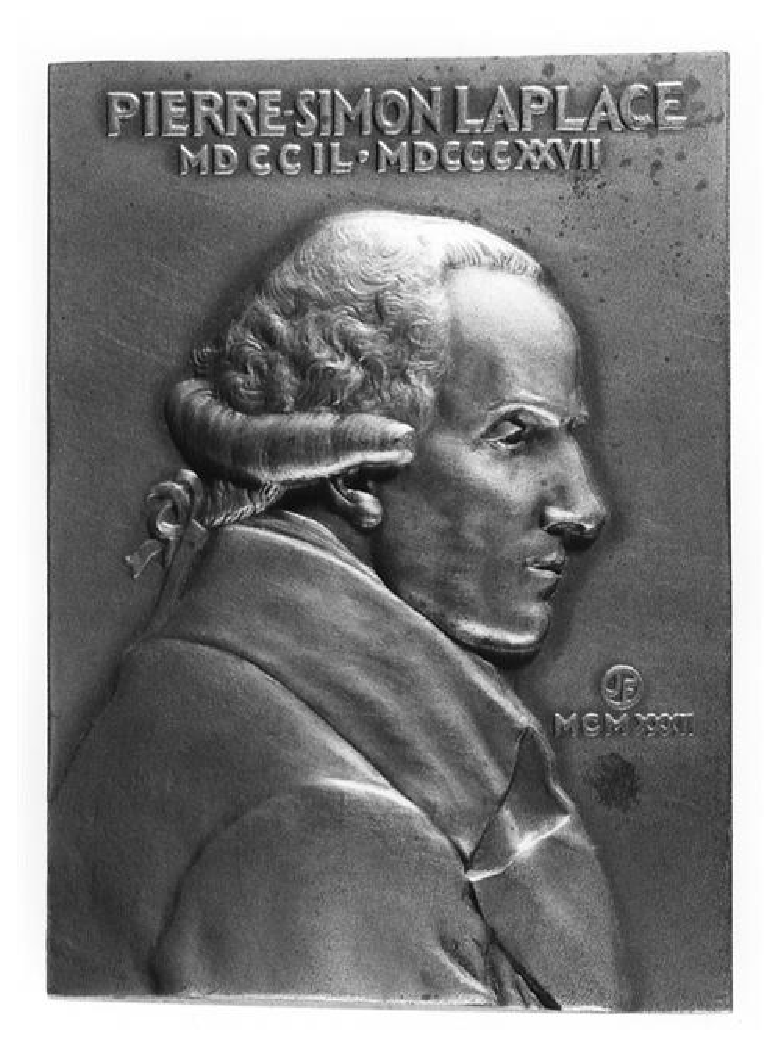
\includegraphics[width=0.9\linewidth]{Pierre-Simon-Laplace_2}
    \caption*{\index{Laplace, Pierre-Simon}\textbf{Pierre-Simon, marquis 
             de Laplace}, (1745-1827) mathématicien, astronome, physicien 
             et homme politique français. (Paris, musée d'Orsay)}
\end{marginfigure}
%-------------------------------------------------------------------------------
%-------------------------------------------------------------------------------
\begin{marginfigure}
    \centering
    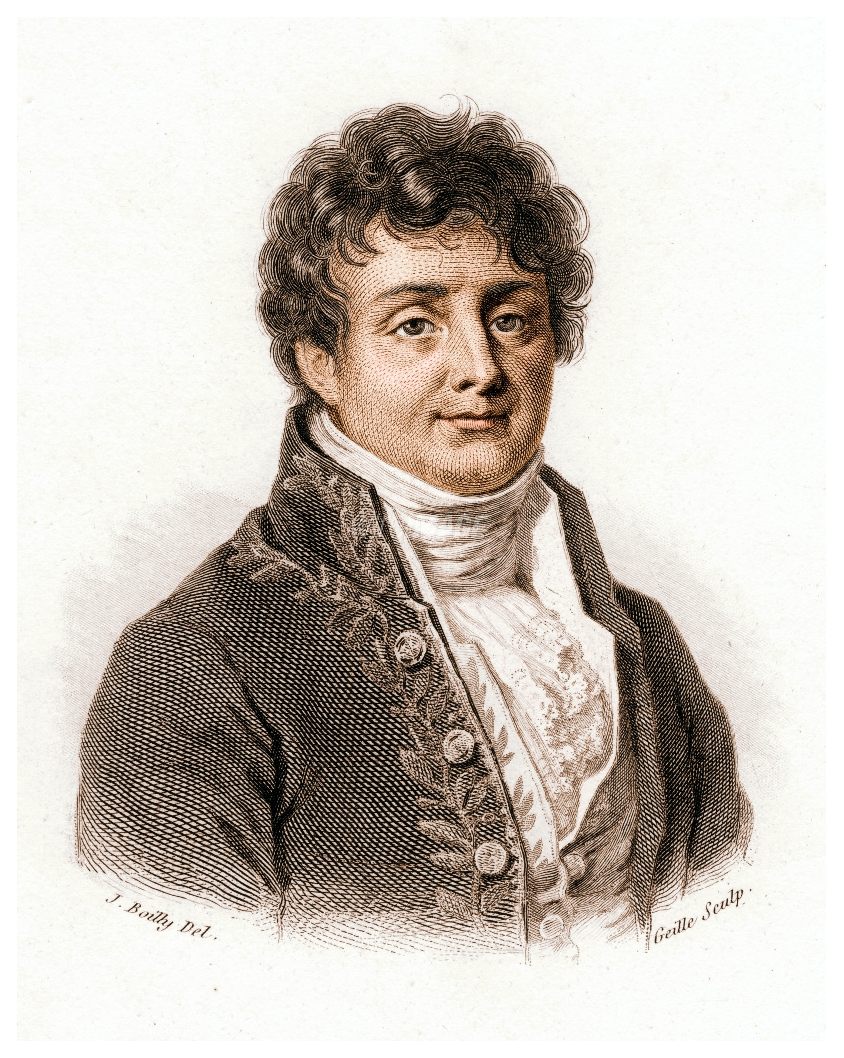
\includegraphics[width=0.9\linewidth]{Fourier}
    \caption*{\index{Fourier, Joseph}\textbf{Jean Baptiste Joseph Fourier}, (1768-1830) mathématicien et physicien 
             français. (Gravure de Julien Léopold Boilly)}
\end{marginfigure}
%-------------------------------------------------------------------------------
%%%%%%%%%%%%%%%%%%%%%%%%%%%%%%%%%%%%%%%%%%%%%%%%%%%%%%%%%%%%%%%%%%%%%%%%%%%%%%%%
%%%%%%%%%%%%%%%%%%%%%%%%%%%%%%%%%%%%%%%%%%%%%%%%%%%%%%%%%%%%%%%%%%%%%%%%%%%%%%%%
\subsection{Définition}
%%%%%%%%%%%%%%%%%%%%%%%%%%%%%%%%%%%%%%%%%%%%%%%%%%%%%%%%%%%%%%%%%%%%%%%%%%%%%%%%
%%%%%%%%%%%%%%%%%%%%%%%%%%%%%%%%%%%%%%%%%%%%%%%%%%%%%%%%%%%%%%%%%%%%%%%%%%%%%%%%
\index{Transformée de Laplace}
La~\gls{tl}, notée $\mathscr{L}$, d'un signal causal $s$ 
fonction d'une variable réelle $t$, est la fonction $S$ 
de la variable complexe $p$, définie par :
%-------------------------------------------------------------------------------
\begin{bequation}[ams align]
S(p)=\laplace{s(t)}=\int_{0}^{+\infty} e^{-pt}s(t)\dd{t}.\label{eq-lap}
\end{bequation}
%-------------------------------------------------------------------------------
On dit également que \textbf{$S(p)$ est l'image dans le domaine de 
Laplace de la fonction $s(t)$ définie dans le domaine temporel.}
Remarquons, dès à présent l'utilisation d'une convention utile: 
\textbf{les fonctions du temps seront toujours désignées par une
minuscule, et les fonctions complexes par la majuscule respective}.
Notons que la transformée de Laplace n'est valide que lorsque la partie réelle 
de p est plus grande qu'une certaine valeur réelle $\alpha$, que l'on nomme 
l'abscisse de convergence avec $-\infty\le\alpha\le+\infty$.

La transformée $S(p)$ de $s(t)$ étant unique, connaissant $S(p)$ on 
en déduit $s(t)$ par la transformation inverse 
\[
    s(t)=\laplacei{S(p)}
\]
Il existe une forme analytique de la transformée inverse basée sur
la formule de Mellin-Fourier\cite{Ostertag}:
\[
    s(t)=\laplacei{S(p)}=\int_{c-j\infty}^{c+j\infty} e^{pt}S(p)\dd{p}
\]
L'intégration de celle-ci est difficile à mettre en oeuvre\footnote{
Il existe différentes méthodes numériques de transformée de Laplace 
inverse (\cref{annexe-invL}). Ces méthodes, hors programme, peuvent 
cependant faire l'objet d'un projet numérique intéressant.}, 
on préferera l'utilisation des tables de transformations de Laplace pour 
réaliser la correspondance inverse (\cref{annexe-lap}). Lorsque la 
transformation n'existe pas dans les tables, il est possible de 
réaliser une décompostion en éléments simples de la réponse $S(p)$ pour 
se placer dans un cas usuel (\cref{annexe-DES}).
\newpage
\restoregeometry
\captionsetup{width=0.9\linewidth,labelfont=bf}
%%%%%%%%%%%%%%%%%%%%%%%%%%%%%%%%%%%%%%%%%%%%%%%%%%%%%%%%%%%%%%%%%%%%%%%%%%%%%%%%
%%%%%%%%%%%%%%%%%%%%%%%%%%%%%%%%%%%%%%%%%%%%%%%%%%%%%%%%%%%%%%%%%%%%%%%%%%%%%%%%
\subsection{Propriétés}
%%%%%%%%%%%%%%%%%%%%%%%%%%%%%%%%%%%%%%%%%%%%%%%%%%%%%%%%%%%%%%%%%%%%%%%%%%%%%%%%
%%%%%%%%%%%%%%%%%%%%%%%%%%%%%%%%%%%%%%%%%%%%%%%%%%%%%%%%%%%%%%%%%%%%%%%%%%%%%%%%
Nous allons ici uniquement présenter les principales propriétés de la TL, 
on se rapportera à nouveau à l'\cref{annexe-lap} pour 
une liste exhaustive de ces propriétés.
%%%%%%%%%%%%%%%%%%%%%%%%%%%%%%%%%%%%%%%%%%%%%%%%%%%%%%%%%%%%%%%%%%%%%%%%%%%%%%%%
\paragraph{Linéarité}
%%%%%%%%%%%%%%%%%%%%%%%%%%%%%%%%%%%%%%%%%%%%%%%%%%%%%%%%%%%%%%%%%%%%%%%%%%%%%%%%
La propriété fondamentale de la transformée de Laplace est d'être linéaire.
Soit deux signaux $s_1(t)$, $s_2(t)$ continus et $S_1(p)$, $S_2(p)$ leurs
transformées de Laplace respectives. La transformée de Laplace d'une 
d'une combinaison linéaire quelconque de $s_1(t)$, $s_2(t)$ est la même 
combinaison linéaire de $S_1(p)$ et $S_2(p)$. Autrement dit,
%-------------------------------------------------------------------------------
\begin{bequation}[ams align]
    \laplace{as_1(t)+bs_2(t)}=aS_1(p)+bS_2(p)
\end{bequation}
%-------------------------------------------------------------------------------
%%%%%%%%%%%%%%%%%%%%%%%%%%%%%%%%%%%%%%%%%%%%%%%%%%%%%%%%%%%%%%%%%%%%%%%%%%%%%%%%
\paragraph{Retard en $t$ (temporel)}
%%%%%%%%%%%%%%%%%%%%%%%%%%%%%%%%%%%%%%%%%%%%%%%%%%%%%%%%%%%%%%%%%%%%%%%%%%%%%%%%
Soit $s(t-\tau)$, un signal $s(t)$ présentant un retard $\tau$.
\[
    \laplace{s(t-\tau)}=\int_{0}^{+\infty} e^{-pt}s(t-\tau)\dd{t}
\]
en appliquant le changement de variable $t'=t-\tau$, on obtient $t=t'+\tau$ 
et $\dd{t}=\dd{t}$
\[
\laplace{s(t-\tau)}
=\int_{\tau}^{+\infty} e^{-p(t'+\tau)}s(t')\dd{t'}
=e^{-p\tau}\int_{0}^{+\infty} e^{-pt'}s(t')\dd{t'}
\]
on reconnaît dans cette dernière expression la définition de la 
transformée de Laplace, on écrit alors :
%-------------------------------------------------------------------------------
\begin{bequation}[ams align]
    \laplace{s(t-\tau)}=e^{-p\tau}S(p)
\end{bequation}
%-------------------------------------------------------------------------------
%%%%%%%%%%%%%%%%%%%%%%%%%%%%%%%%%%%%%%%%%%%%%%%%%%%%%%%%%%%%%%%%%%%%%%%%%%%%%%%%
\paragraph{Retard en $p$ (Thèorème de l'amortissement)}
%%%%%%%%%%%%%%%%%%%%%%%%%%%%%%%%%%%%%%%%%%%%%%%%%%%%%%%%%%%%%%%%%%%%%%%%%%%%%%%%
Soit $s(t)$ un signal de transformée de Laplace $S(p)$. La transformée 
de Laplace du signal modifié $e^{-at}s(t)$ s'écrit :
\[
\laplace{e^{-at}s(t)}
=\int_{0}^{+\infty} e^{-pt}e^{-at}s(t)\dd{t}
=\int_{0}^{+\infty} e^{-(p+a)t}s(t)\dd{t}
\]
on reconnaît dans cette dernière expression la définition de la transformée 
de Laplace pour $p+a$, on obtient donc la transformée, 
%-------------------------------------------------------------------------------
\begin{bequation}[ams align]
    \laplace{e^{-at}s(t)}=S(p+a)
\end{bequation}
%-------------------------------------------------------------------------------
ou encore,
%-------------------------------------------------------------------------------
\begin{bequation}[ams align]
    \laplacei{S(p+a)}=e^{-at}s(t).
\end{bequation}
%-------------------------------------------------------------------------------
%%%%%%%%%%%%%%%%%%%%%%%%%%%%%%%%%%%%%%%%%%%%%%%%%%%%%%%%%%%%%%%%%%%%%%%%%%%%%%%%
\paragraph{Dérivation}
%%%%%%%%%%%%%%%%%%%%%%%%%%%%%%%%%%%%%%%%%%%%%%%%%%%%%%%%%%%%%%%%%%%%%%%%%%%%%%%%
Soit un signal $s(t)$ continu et dérivable pour $t\ge0$ et $S(p)$ 
sa transformée de Laplace. Par définition de la transformée de Laplace 
\[
\laplace{\devi{s(t)}{}}=\int_{0}^{+\infty} e^{-pt}\devi{s(t)}{}\dd{t}
\]
par intégration par parties
%-------------------------------------------------------------------------------
\begin{align*}
    v=e^{-pt}\qquad&\dd{u}=\devi{s(t)}{}\dd{t}\\
    \dd{v}=-pe^{-pt}\dd{t}\qquad&u=s(t)
\end{align*}
%-------------------------------------------------------------------------------
%-------------------------------------------------------------------------------
\begin{align*}
\laplace{\devi{s(t)}{}}&=\left[s(t)e^{-pt}\right]_0
                         ^{+\infty}-p\int_{0}^{+\infty}e^{-pt}s(t)\dd{t}\\
                         &=-s(0)+pS(p)
\end{align*}
%-------------------------------------------------------------------------------
ou encore
%-------------------------------------------------------------------------------
\begin{bequation}[ams align]
    \laplace{\devi{s(t)}{}}=pS(p)-s(0)
\end{bequation}
%-------------------------------------------------------------------------------
On généralise à tous les ordres de dérivation dans le cas de conditions 
initiales nulles.
\[
\laplace{\devi{s(t)}{n}}=p^nS(p)
\]
Remarquons alors que \textbf{dériver dans le domaine temporel consiste 
à multiplier par $p$ dans le domaine de Laplace.}
%%%%%%%%%%%%%%%%%%%%%%%%%%%%%%%%%%%%%%%%%%%%%%%%%%%%%%%%%%%%%%%%%%%%%%%%%%%%%%%%
\paragraph{Intégration}
%%%%%%%%%%%%%%%%%%%%%%%%%%%%%%%%%%%%%%%%%%%%%%%%%%%%%%%%%%%%%%%%%%%%%%%%%%%%%%%%
Soient  des signaux $v(t)$ et $s(t)$ tel que 
$v(t)=\int_{0}^{t}s(\tau)\dd{\tau}$. Par définition,
\[
\laplace{v(t)}=\int_{0}^{+\infty} e^{-pt}v(t)\dd{t}
\]
par intégration par parties,
%-------------------------------------------------------------------------------
\begin{align*}
    v=v(t)\qquad&\dd{u}=e^{-pt}\dd{t}\\
    \dd{v}=s(t)\dd{t}\qquad&u=-\dfrac{1}{p}e^{-pt}
\end{align*} 
%-------------------------------------------------------------------------------
\begin{align*}
    \laplace{v(t)}&=\left[-\dfrac{1}{p}v(t)e^{-pt}\right]_0^{+\infty}
                          -\int_{0}^{+\infty}
                          -\dfrac{1}{p}e^{-pt}s(t)\dd{t} \\
    &=\dfrac{1}{p}\int_{0}^{+\infty} e^{-pt}s(t)\dd{t}+\dfrac{s(0)}{p}
\end{align*}
%-------------------------------------------------------------------------------
ou encore
%-------------------------------------------------------------------------------
\begin{bequation}[ams align]
    \laplace{\int_{0}^{t}s(\tau)\dd{\tau}}=\dfrac{S(p)}{p}+\dfrac{s(0)}{p}
\end{bequation}
%-------------------------------------------------------------------------------
Remarquons alors que \textbf{intégrer dans le domaine temporel consiste à 
diviser par $p$ dans le domaine de Laplace.}
%%%%%%%%%%%%%%%%%%%%%%%%%%%%%%%%%%%%%%%%%%%%%%%%%%%%%%%%%%%%%%%%%%%%%%%%%%%%%%%%
\paragraph{Théorème de la valeur initiale}
%%%%%%%%%%%%%%%%%%%%%%%%%%%%%%%%%%%%%%%%%%%%%%%%%%%%%%%%%%%%%%%%%%%%%%%%%%%%%%%%
\index{Théorème!de la valeur initiale}
%-------------------------------------------------------------------------------
\begin{bequation}[ams align]
    s(0)=\lim\limits_{p\rightarrow+\infty} p S(p)\qquad \forall S(p)
\end{bequation}
%-------------------------------------------------------------------------------
où $s(0)$ est la valeur d'un signal $s(t)$ pour $t=0$.
Ce théorème est utilisé pour déterminer la valeur initiale
dans le domaine temporelle d'un signal dont on connait 
uniquement la transformée de Laplace.
%%%%%%%%%%%%%%%%%%%%%%%%%%%%%%%%%%%%%%%%%%%%%%%%%%%%%%%%%%%%%%%%%%%%%%%%%%%%%%%%
\paragraph{Théorème de la valeur finale}
%%%%%%%%%%%%%%%%%%%%%%%%%%%%%%%%%%%%%%%%%%%%%%%%%%%%%%%%%%%%%%%%%%%%%%%%%%%%%%%%
\index{Théorème!de la valeur finale}
%-------------------------------------------------------------------------------
\begin{bequation}[ams align]
    s(\infty)=\lim\limits_{p\rightarrow0} p S(p)
\end{bequation}
%-------------------------------------------------------------------------------
où $s(\infty)$ est la valeur d'un signal $s(t)$ pour $t\to\infty$.
Ce théorème n'est valable que si $s(\infty)$ est définie. Ou comme on le 
dira plus tard si le signal est stable.
%%%%%%%%%%%%%%%%%%%%%%%%%%%%%%%%%%%%%%%%%%%%%%%%%%%%%%%%%%%%%%%%%%%%%%%%%%%%%%%%
\paragraph{Transformée de Laplace d'un produit de convolution}
%%%%%%%%%%%%%%%%%%%%%%%%%%%%%%%%%%%%%%%%%%%%%%%%%%%%%%%%%%%%%%%%%%%%%%%%%%%%%%%%
Le produit de convolution de deux signaux $h(t)$ et $e(t)$ que l'on 
note $(h*e)(t)$ est défini par :
\[
    (h*e)(t)=\int_{-\infty}^{+\infty}h(t-\tau)e(\tau)\dd{\tau}
\]
La transformée de Laplace transforme le produit de convolution en un simple
produit des signaux dans le domaine de Laplace. Formellement,
%-------------------------------------------------------------------------------
\begin{bequation}[ams align]
    \laplace{(h*e)(t)}=H(p)E(p)
\end{bequation}
%-------------------------------------------------------------------------------
Si cette propriété est fondamentale, nous ne l'utiliserons 
que très exceptionnellement. Nous la rencontrerons à nouveau, 
dans ce chapitre, lorsque nous introduierons la fonction de 
transfert d'un système linéaire.
%%%%%%%%%%%%%%%%%%%%%%%%%%%%%%%%%%%%%%%%%%%%%%%%%%%%%%%%%%%%%%%%%%%%%%%%%%%%%%%%
%%%%%%%%%%%%%%%%%%%%%%%%%%%%%%%%%%%%%%%%%%%%%%%%%%%%%%%%%%%%%%%%%%%%%%%%%%%%%%%%
\subsection{Transformées des signaux usuels}
%%%%%%%%%%%%%%%%%%%%%%%%%%%%%%%%%%%%%%%%%%%%%%%%%%%%%%%%%%%%%%%%%%%%%%%%%%%%%%%%
%%%%%%%%%%%%%%%%%%%%%%%%%%%%%%%%%%%%%%%%%%%%%%%%%%%%%%%%%%%%%%%%%%%%%%%%%%%%%%%%
Nous présentons les transformées de Laplace des signaux usuels introduits
au paragraphe~\ref{sec-signaux_usuels}
%%%%%%%%%%%%%%%%%%%%%%%%%%%%%%%%%%%%%%%%%%%%%%%%%%%%%%%%%%%%%%%%%%%%%%%%%%%%%%%%
\paragraph{Transformée d'une impulsion de Dirac}
%%%%%%%%%%%%%%%%%%%%%%%%%%%%%%%%%%%%%%%%%%%%%%%%%%%%%%%%%%%%%%%%%%%%%%%%%%%%%%%%
\index{Transformée de Laplace!d'une impulsion de Dirac}
Par simple application des définitions 
de la~\gls{tl} et de l'impulsion de Dirac, la transformée d'une 
impulsion de Dirac $\delta(t)$ s'écrit:
\[
    \laplace{\delta(t)}=\int_{0}^{+\infty} e^{-pt}\,\delta(t)\dd{t}=1
\]
ou encore
%-------------------------------------------------------------------------------
\begin{bequation}[ams align]
    \laplace{\delta(t)}=1
\end{bequation}
%-------------------------------------------------------------------------------
%%%%%%%%%%%%%%%%%%%%%%%%%%%%%%%%%%%%%%%%%%%%%%%%%%%%%%%%%%%%%%%%%%%%%%%%%%%%%%%%
\paragraph{Transformée d'un échelon-unité}
%%%%%%%%%%%%%%%%%%%%%%%%%%%%%%%%%%%%%%%%%%%%%%%%%%%%%%%%%%%%%%%%%%%%%%%%%%%%%%%%
\index{Transformée de Laplace!d'un échelon-unité}
La transformée de Laplace d'un signal échelon-unité  s'écrit : 
\[
\laplace{u(t)}=\int_{0}^{+\infty}e^{-pt}\,u(t)\dd{t}
=\int_{0}^{+\infty} e^{-pt}\dd{t}
=\left[\dfrac{-e^{-pt}}{p}\right]_0^{+\infty}=\dfrac{1}{p}
\]
ou encore
%-------------------------------------------------------------------------------
\begin{bequation}[ams align]
    \laplace{u(t)}=\dfrac{1}{p}
\end{bequation}
%-------------------------------------------------------------------------------
Dans le cas de la forme généralisée, il suffit de multiplier par une constante.
%%%%%%%%%%%%%%%%%%%%%%%%%%%%%%%%%%%%%%%%%%%%%%%%%%%%%%%%%%%%%%%%%%%%%%%%%%%%%%%%
\paragraph{Transformée d'une rampe}
%%%%%%%%%%%%%%%%%%%%%%%%%%%%%%%%%%%%%%%%%%%%%%%%%%%%%%%%%%%%%%%%%%%%%%%%%%%%%%%%
\index{Transformée de Laplace!d'une rampe}
La transformée de Laplace d'un signal rampe s'écrit :
\[
\laplace{r(t)}=\int_{0}^{+\infty} e^{-pt}r(t)\dd{t}
=\int_{0}^{+\infty} te^{-pt}\dd{t}
\]
Par intégration par parties:
%-------------------------------------------------------------------------------
\begin{align*}
    v=-\dfrac{1}{p}e^{-pt}\qquad&\dd{u}=\dd{t}\\
    \dd{v}=e^{-pt}\dd{t}\qquad&u=t
\end{align*}
%-------------------------------------------------------------------------------
\[
\int_{0}^{+\infty} te^{-pt}\dd{t}
=\left[-t\dfrac{1}{p}e^{-pt}\right]_0^{+\infty}-\int_{0}^{+\infty}
-\dfrac{1}{p}e^{-pt}\dd{t}=\dfrac{1}{p^2}
\]
ou encore
%-------------------------------------------------------------------------------
\begin{bequation}[ams align]
    \laplace{r(t)}=\laplace{t\cdot u(t)}=\dfrac{1}{p^2}.
\end{bequation}
%-------------------------------------------------------------------------------
On généralise aux ordres supérieures (\og parabolique\fg, \og 
cubique\fg\ldots) :
%-------------------------------------------------------------------------------
\begin{bequation}[ams align]
    \laplace{\dfrac{1}{n!}t^n\cdot u(t)}=\dfrac{1}{p^{n+1}}.
\end{bequation}
%-------------------------------------------------------------------------------
%%%%%%%%%%%%%%%%%%%%%%%%%%%%%%%%%%%%%%%%%%%%%%%%%%%%%%%%%%%%%%%%%%%%%%%%%%%%%%%%
\paragraph{Transformée d'une exponentielle décroissante}
%%%%%%%%%%%%%%%%%%%%%%%%%%%%%%%%%%%%%%%%%%%%%%%%%%%%%%%%%%%%%%%%%%%%%%%%%%%%%%%%
\index{Transformée de Laplace!d'une exponentielle décroissante}
La transformée de Laplace d'une exponentielle décroissante s'écrit :
\[
\laplace{e^{-at}u(t)}=\int_{0}^{+\infty} e^{-pt}e^{-at}\dd{t}
=\int_{0}^{+\infty} e^{-(p+a)t}\dd{t} = \dfrac{1}{p+a}
\]
ou encore
%-------------------------------------------------------------------------------
\begin{bequation}[ams align]
    \laplace{e^{-at}u(t)}=\dfrac{1}{p+a}
\end{bequation}
%-------------------------------------------------------------------------------
Nous aurions pu utiliser la propriété du retard en $p$ 
(Théorème de l'amortissement) pour déterminer cette transformée de Laplace.
%%%%%%%%%%%%%%%%%%%%%%%%%%%%%%%%%%%%%%%%%%%%%%%%%%%%%%%%%%%%%%%%%%%%%%%%%%%%%%%%
\paragraph{Transformée d'un sinus}
%%%%%%%%%%%%%%%%%%%%%%%%%%%%%%%%%%%%%%%%%%%%%%%%%%%%%%%%%%%%%%%%%%%%%%%%%%%%%%%%
\index{Transformée de Laplace!d'un sinus}
La transformée de Laplace de la fonction sinus s'écrit :
%-------------------------------------------------------------------------------
\begin{align*}
\laplace{\sin{\omega t}\cdot u(t)}&=
\int_{0}^{+\infty}e^{-pt}\dfrac{e^{\jw t}-e^{-\jw t}}{2j}\dd{t}\\
&=\dfrac{1}{2j}\int_{0}^{+\infty}e^{-(p-\jw)t}\dd{t} - 
  \dfrac{1}{2j}\int_{0}^{+\infty}e^{-(p+\jw)t}\dd{t} \\
&=\dfrac{1}{2j}\left( \dfrac{1}{p-\jw}-\dfrac{1}{p+\jw}\right)\\
&=\dfrac{\omega}{p^2+\omega^2}
\end{align*}
%-------------------------------------------------------------------------------
ou encore
%-------------------------------------------------------------------------------
\begin{bequation}[ams align]
    \laplace{\sin{\omega t}\cdot u(t)}=\dfrac{\omega}{p^2+\omega^2}
\end{bequation}
%-------------------------------------------------------------------------------
%%%%%%%%%%%%%%%%%%%%%%%%%%%%%%%%%%%%%%%%%%%%%%%%%%%%%%%%%%%%%%%%%%%%%%%%%%%%%%%%
\paragraph{Transformée d'un cosinus}
%%%%%%%%%%%%%%%%%%%%%%%%%%%%%%%%%%%%%%%%%%%%%%%%%%%%%%%%%%%%%%%%%%%%%%%%%%%%%%%%
\index{Transformée de Laplace!d'un cosinus}
La transformée de Laplace de la fonction cosinus s'écrit :
%-------------------------------------------------------------------------------
\begin{align*}
\laplace{\cos{\omega t}\cdot u(t)}&=\int_{0}^{+\infty}e^{-pt}
\dfrac{e^{\jw t}+e^{-\jw t}}{2}\dd{t}\\
&=\dfrac{1}{2}\int_{0}^{+\infty}e^{-(p-\jw)t}\dd{t} + 
\dfrac{1}{2j}\int_{0}^{+\infty}e^{-(p+\jw)t}\dd{t} \\
&=\dfrac{1}{2}\left( \dfrac{1}{p-\jw}+\dfrac{1}{p+\jw}\right)\\
&=\dfrac{p}{p^2+\omega^2}
\end{align*}
%-------------------------------------------------------------------------------
ou encore
%-------------------------------------------------------------------------------
\begin{bequation}[ams align]
    \laplace{\cos{\omega t}\cdot u(t)}=\dfrac{p}{p^2+\omega^2}
\end{bequation}
%-------------------------------------------------------------------------------
\newpage
\input{re/newgeometry}
\captionsetup{width=0.9\linewidth,labelfont=bf}
%%%%%%%%%%%%%%%%%%%%%%%%%%%%%%%%%%%%%%%%%%%%%%%%%%%%%%%%%%%%%%%%%%%%%%%%%%%%%%%%
%%%%%%%%%%%%%%%%%%%%%%%%%%%%%%%%%%%%%%%%%%%%%%%%%%%%%%%%%%%%%%%%%%%%%%%%%%%%%%%%
\subsection[Application de la transformée de Laplace]
           {Application de la TL à la résolution d'équation différentielle}
%%%%%%%%%%%%%%%%%%%%%%%%%%%%%%%%%%%%%%%%%%%%%%%%%%%%%%%%%%%%%%%%%%%%%%%%%%%%%%%%
%%%%%%%%%%%%%%%%%%%%%%%%%%%%%%%%%%%%%%%%%%%%%%%%%%%%%%%%%%%%%%%%%%%%%%%%%%%%%%%%
%-------------------------------------------------------------------------------
\begin{figure}[!ht]
    \centering
    \tikzsetnextfilename{laplace_schema-chap_slci-ext}
    \begin{tikzpicture}
\tikzset{both/.style={draw,minimum width=4cm,minimum height=2cm,rounded corners=.1cm,inner sep=0.5pt,text width=4cm,align=center}}
\tikzstyle{temp}=[both,fill=blue!25!white]
\tikzstyle{lapl}=[both,fill=red!25!white]
\node[temp] (a) at (0,0)  {\small\'Equation différentielle\\ (domaine temporel)};
\node[temp] (b) at (7,0)  {\small Solution \\(domaine temporel)};
\node[lapl] (c) at  (0,-4){\small \'Equation algébrique\\ (domaine de Laplace)};
\node[lapl] (d) at (7,-4) {\small Solution \\(domaine de Laplace)};
\draw[very thick,-{Latex[length=3.5mm]}] (a) --node[above,align=center,text width=2cm] {Résolution\\direct} (b);
\draw[very thick,-{Latex[length=3.5mm]}] (d) --node[right] {\Large$\mathscr{L}^{-1}$} (b);
\draw[very thick,-{Latex[length=3.5mm]}] (a) --node[left] {\Large$\mathscr{L}$} (c);
\draw[very thick,-{Latex[length=3.5mm]}] (c) --node[below,align=center,text width=2cm] {Résolution\\algébrique} (d);
\end{tikzpicture}



    \caption{Représentation schématique de la méthode employée pour la 
             résolution des équations différentielles linéaires à 
             coefficients constants.\label{fig-laplace_schema}}
\end{figure}
%-------------------------------------------------------------------------------
%%%%%%%%%%%%%%%%%%%%%%%%%%%%%%%%%%%%%%%%%%%%%%%%%%%%%%%%%%%%%%%%%%%%%%%%%%%%%%%%
\subsubsection{Méthodologie}
%%%%%%%%%%%%%%%%%%%%%%%%%%%%%%%%%%%%%%%%%%%%%%%%%%%%%%%%%%%%%%%%%%%%%%%%%%%%%%%%
Lorsqu'une équation différentielle à coefficients constants a pu être établie
pour définir la relation entre l'entrée et la sortie d'un \gls{slci}, il 
nous faut en trouver une solution. Les méthodes classiques de résolution 
d'équations différentielles peuvent être difficiles et fastidieuses à mettre 
en oeuvre, notamment dans le cas d'équation différentielle d'ordre élevé 
ou encore pour des systèmes composés de sous-systèmes.

La transformée de Laplace permet de mettre en oeuvre une méthode plus simple et 
systèmatique  pour la la résolution de ces équations différentielles à 
coefficients constants.

Comme nous l'avons déjà discuté, la forme générale de ces équations est 
donnée par :
%-------------------------------------------------------------------------------
\begin{align}
    \sum_{i=0}^{n}a_i\devi{s(t)}{i}=\sum_{i=0}^{m}b_i\devi{e(t)}{i}
    \label{eq-ltemp}
\end{align}
%-------------------------------------------------------------------------------
avec $n,m\in\mathbb{N}$, $s(t)$ le signal de sortie, $e(t)$ le signal 
d'entrée et $a_i,b_i\in\mathbb{R}$. L'équation est dite d'ordre $n$.
%-------------------------------------------------------------------------------
\begin{marginfigure}
    \centering
    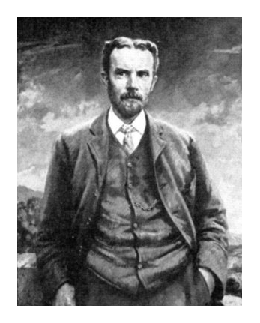
\includegraphics[width=0.9\linewidth]{OliverHeaviside.eps}
    \caption*{\index{Heaviside, Oliver}\textbf{Oliver Heaviside} (1850-1925), 
              physicien britannique. Il développa le calcul opérationnel 
              pour résoudre les équations différentielles}.
\end{marginfigure}
%-------------------------------------------------------------------------------
Sous cette forme, cette équation différentielle constitue ce que l'on 
nomme \textbf{la loi temporelle} du système. Sans perte de généralité, on ne 
considèrera dans un premier temps que les systèmes pour lesquels toutes les 
\textbf{conditions initialles sont nulles}, appelées également les conditions 
d'Heaviside
\newpage
\restoregeometry
\captionsetup{width=0.9\linewidth,labelfont=bf}
En appliquant la transformée de Laplace à l'\cref{eq-ltemp}, on obtient 
ce que l'on nomme \textbf{la loi fréquentielle} du système :
%-------------------------------------------------------------------------------
\begin{bequation}[ams align]
    \sum_{i=0}^{n}a_ip^iS(p)=\sum_{i=0}^{m}b_ip^iE(p)\label{eq-lfreq}
\end{bequation}
%-------------------------------------------------------------------------------
La résolution algébrique de cette équation est simplement donnée par :
%-------------------------------------------------------------------------------
\begin{bequation}[ams align]
    S(p)=\dfrac{\sum\limits_{i=0}^{m}b_ip^i}
    {\sum\limits_{i=0}^{n}a_ip^i}E(p)\label{eq-lfreq2}
\end{bequation}
%-------------------------------------------------------------------------------
La solution dans le domaine temporelle $s(t)$ de l'équation différentielle 
est alors simplement obtenue par transformée de Laplace inverse de $S(p)$.

Cette méthode, résumée par l'organigramme de la~\cref{fig-laplace_schema}, 
est appliqué à un exemple complet au paragraphe suivant.
%%%%%%%%%%%%%%%%%%%%%%%%%%%%%%%%%%%%%%%%%%%%%%%%%%%%%%%%%%%%%%%%%%%%%%%%%%%%%%%%
\subsubsection{Exemple complet}
%%%%%%%%%%%%%%%%%%%%%%%%%%%%%%%%%%%%%%%%%%%%%%%%%%%%%%%%%%%%%%%%%%%%%%%%%%%%%%%%
Soit l'équation différentielle suivante :
%-------------------------------------------------------------------------------
\begin{align}
\devi{s(t)}{2}+2\devi{s(t)}{} + s(t) = e(t)\label{eq-diff1}
\end{align}
%-------------------------------------------------------------------------------
où $e(t)$ et $s(t)$ sont respectivement les fonctions temporelles de l'entrée 
et de la sortie du système régi par cette équation différentielle. 
Nous considérons la réponse à un échelon-unité (c.-à-d. $e(t)=u(t)$ ) 
avec pour conditions initiales :
%-------------------------------------------------------------------------------
\begin{align*}
    s(0) &=-1\\
    s'(0)&=2.
\end{align*}
%-------------------------------------------------------------------------------
Nous allons résoudre cette équation par deux méthodes différentes: 
\textbf{la méthode direct de résolution d'équations différentielles avec 
second membre}, et par l'\textbf{application de la transformée de Laplace}.
Nous pourrons observer que l'application de la TL pour la résolution
des équations différentielles est une méthode plus systèmatique qui 
s'affranchit de la forme particulière de l'équation différentielle 
auquelle on a à faire. Nous verrons que la transformée de Laplace devient 
totalement indispensable pour la caractérisation d'un \gls{slci}.
\newpage
\input{re/newgeometry}
\captionsetup{width=0.9\linewidth,labelfont=bf}
%%%%%%%%%%%%%%%%%%%%%%%%%%%%%%%%%%%%%%%%%%%%%%%%%%%%%%%%%%%%%%%%%%%%%%%%%%%%%%%%
\paragraph{Résolution par la méthode direct}
%%%%%%%%%%%%%%%%%%%%%%%%%%%%%%%%%%%%%%%%%%%%%%%%%%%%%%%%%%%%%%%%%%%%%%%%%%%%%%%%
L'équation caractéristique associée à cette équation différentielle est 
donnée par 
\[
    r^2+2r+1=0
\]
cette équation possède une solution double $r_{1,2}=-1$.
La solution générale de l'équation homogène $s_0(t)$ (c.a.d sans second membre) 
est donc de la forme :
\[
    s_0(t)=(\alpha t+\beta)e^{-t}.
\]
Une solution particulière $s_1(t)=1$ nous est trivialement donnée par l'entrée 
en échelon qui correspond au régime permanent.
La solution générale est donc donnée par :
\[
    s(t)=(\alpha t+\beta)e^{-t}+1
\]
Dérivons cette solution générale pour pouvoir déterminer les coefficients 
$\alpha$, $\beta$ en utilisant les conditions initiales,
%-------------------------------------------------------------------------------
\begin{align*}
    s'(t)&=\alpha e^{-t}-(\alpha t+\beta)e^{-t}\\
     s(0)&=-1\Rightarrow\beta+1=-1\Rightarrow\beta=-2 \\
    s'(0)&=\hphantom{-}2\Rightarrow\alpha+2=\hphantom{-}2\Rightarrow\alpha=0
\end{align*}
%-------------------------------------------------------------------------------
La solution générale de l'équation différentielle~(\ref{eq-diff1}) est 
donc donnée par 
%-------------------------------------------------------------------------------
\begin{marginfigure}
    \centering
    \tikzsetnextfilename{sol_eq_diff-chap_slci-ext}
    \resizebox{\linewidth}{!}{\input{tikz/sol_eq_diff-chap_slci.tex}}
    \caption{Représentation de la solution générale de l'équation 
             différentielle~(\ref{eq-diff1}) pour $e(t)=u(t)$. 
             On vérifie lors du tracé que l'on observe bien les principales 
             propriétes du signal (c.-à-d. conditions initiales, 
             valeur finale).\label{fig-solution}}
\end{marginfigure}
%-------------------------------------------------------------------------------
%-------------------------------------------------------------------------------
\begin{bequation}[ams align]
s(t)=1-2e^{-t}.
\end{bequation}
%-------------------------------------------------------------------------------
Nous laissons au lecteur le soin de vérifier que cette fonction est solution 
de l'équation~\ref{eq-diff1}, et qu'elle respecte notamment les conditions 
initiales. Le graphe de la solution est également présenté 
(\Cref{fig-solution}).
%%%%%%%%%%%%%%%%%%%%%%%%%%%%%%%%%%%%%%%%%%%%%%%%%%%%%%%%%%%%%%%%%%%%%%%%%%%%%%%%
\paragraph{Résolution par application de la transformée de Laplace}
%%%%%%%%%%%%%%%%%%%%%%%%%%%%%%%%%%%%%%%%%%%%%%%%%%%%%%%%%%%%%%%%%%%%%%%%%%%%%%%%
\index{Transformée de Laplace! résolution d'équation différentielle}
La transformée de Laplace est linéaire. Il nous est alors possible
de l'appliquer aux différents termes de l'équation 
différentielle~(\ref{eq-diff1}) séparément.
On obtient pour chacun des termes :
%-------------------------------------------------------------------------------
\begin{align*}
    \laplace{s(t)} &= S(p), \\
    \laplace{\devi{s(t)}{}} &= pS(p)-s(0) = pS(p) +1, \\
    \laplace{\devi{s(t)}{2}} &= p^2S(p)-ps(0)-s'(0) = p^2S(p) + p -2,\\
    \laplace{u(t)} &= \dfrac{1}{p}.
\end{align*}
%-------------------------------------------------------------------------------
\newpage
\restoregeometry
\captionsetup{width=0.9\linewidth,labelfont=bf}
L'équation différentielle~(\ref{eq-diff1}) devient dans le domaine 
de Laplace :
%-------------------------------------------------------------------------------
\begin{align*}
p^2S(p)+p-2+2pS(p)+2+S(p)=\dfrac{1}{p} 
\end{align*}
%-------------------------------------------------------------------------------
En réarrangeant cette expression, il est possible de déterminer la 
forme de la réponse $S(p)$ dans le domaine de Laplace.
%-------------------------------------------------------------------------------
\begin{align*}
    S(p)\left(p^2+2p+1\right)+p&=\dfrac{1}{p} \\
    %S(p)\left(p+1\right)^2 &= \dfrac{1-p^2}{p}\\
    S(p)&= \dfrac{1-p^2}{p\left(p+1\right)^2}
\end{align*}
%-------------------------------------------------------------------------------
de Laplace usuels, nous allons décomposer cette
fraction rationnelle en éléments simples (\Cref{annexe-DES}).
\[
    S(p)=\dfrac{A}{p}+\dfrac{B}{p+1}+\dfrac{C}{(p+1)^2}
\]
Par identification, 
\[
    S(p)=\dfrac{A(p+1)^2+Bp(p+1)+Cp}{p(p+1)^2}
        =\dfrac{1-p^2}{p\left(p+1\right)^2}
\]
\[
\begin{cases}
    A+B&=-1 \\
    2A+B+C&=0 \\
    A&=1   
\end{cases}\Rightarrow
\begin{cases}
    B&=-2\\
    C&=0
\end{cases}
\]
La réponse $S(p)$ se décompose donc de la façon suivante en éléments simples:
\[
    S(p)=\dfrac{1}{p}-\dfrac{2}{p+1}
\]
Il est maintenant plus aisé d'appliquer la transformation de Laplace inverse, 
en utilisant le tableau des transformées de Laplace usuels 
(c.f lignes 3 et 7 du tableau de l'\Cref{annexe-lap}) pour obtenir la 
réponse temporelle $s(t)$. Notamment,
\[
    \laplacei{\dfrac{1}{p}}=1
\]
et
\[
    \laplacei{\dfrac{2}{p+1}}=2e^{-t}
\]
soit 
%-------------------------------------------------------------------------------
\begin{bequation}[ams align]
    \laplacei{S(p)}=s(t)=1-2e^{-t}
\end{bequation}
%-------------------------------------------------------------------------------
Comme attendu, les deux méthodes donnent le même résultat, cependant 
la transformée de Laplace permet de définir dans le domaine de Laplace, une 
relation direct entre l'entrée et la sortie d'un système. C'est la fonction 
de transfert qui réalise ce lien.
\clearpage
%%%%%%%%%%%%%%%%%%%%%%%%%%%%%%%%%%%%%%%%%%%%%%%%%%%%%%%%%%%%%%%%%%%%%%%%%%%%%%%%
%%%%%%%%%%%%%%%%%%%%%%%%%%%%%%%%%%%%%%%%%%%%%%%%%%%%%%%%%%%%%%%%%%%%%%%%%%%%%%%%
%%%%%%%%%%%%%%%%%%%%%%%%%%%%%%%%%%%%%%%%%%%%%%%%%%%%%%%%%%%%%%%%%%%%%%%%%%%%%%%%
\section{Fonction de Transfert}
%%%%%%%%%%%%%%%%%%%%%%%%%%%%%%%%%%%%%%%%%%%%%%%%%%%%%%%%%%%%%%%%%%%%%%%%%%%%%%%%
%%%%%%%%%%%%%%%%%%%%%%%%%%%%%%%%%%%%%%%%%%%%%%%%%%%%%%%%%%%%%%%%%%%%%%%%%%%%%%%%
%%%%%%%%%%%%%%%%%%%%%%%%%%%%%%%%%%%%%%%%%%%%%%%%%%%%%%%%%%%%%%%%%%%%%%%%%%%%%%%%
%%%%%%%%%%%%%%%%%%%%%%%%%%%%%%%%%%%%%%%%%%%%%%%%%%%%%%%%%%%%%%%%%%%%%%%%%%%%%%%%
%%%%%%%%%%%%%%%%%%%%%%%%%%%%%%%%%%%%%%%%%%%%%%%%%%%%%%%%%%%%%%%%%%%%%%%%%%%%%%%%
\subsection{Définition}
%%%%%%%%%%%%%%%%%%%%%%%%%%%%%%%%%%%%%%%%%%%%%%%%%%%%%%%%%%%%%%%%%%%%%%%%%%%%%%%%
%%%%%%%%%%%%%%%%%%%%%%%%%%%%%%%%%%%%%%%%%%%%%%%%%%%%%%%%%%%%%%%%%%%%%%%%%%%%%%%%
\index{Fonction de Transfert}
La fonction de transfert $H(p)$ d'un système est donnée par le rapport de la 
sortie $S(p)$ et l'entrée $E(p)$ dans le domaine de Laplace. 
%-------------------------------------------------------------------------------
\begin{bequation}[ams align]
    H(p)=\dfrac{S(p)}{E(p)}
\end{bequation}
%-------------------------------------------------------------------------------
ou encore,
%-------------------------------------------------------------------------------
\begin{bequation}[ams align]
    S(p)=H(p)E(p)\label{eq-she}
\end{bequation}
%-------------------------------------------------------------------------------
Cette fonction $H(p)$, également appelé \textbf{transmittance}, caractérise 
le système de façon univoque. Pour une entrée donnée il est possible de 
prévoir la sortie d'un système caractérisé par sa fonction de transfert $H(p)$.

Nous représenterons très souvent cette relation dans le domaine de Laplace 
par le schéma-bloc suivant : 
%-------------------------------------------------------------------------------
\begin{center}
    \tikzsetnextfilename{sb_bloc_FT-chap_slci-ext}
    \begin{tikzpicture}
    \sbEntree{E1}
    \sbBloc[3]{B1}{$H(p)$}{E1}
    \sbRelier[$E(p)$]{E1}{B1}
    \sbSortie[3]{S1}{B1}
    \sbRelier[$S(p)$]{B1}{S1}
\end{tikzpicture}

\end{center}
%-------------------------------------------------------------------------------
%Cette relation entre la sortie et l'entrée du système dans le domaine de 
%Laplace provient directement de la relation temporelle associée à l'équation 
%différentielle du phénomène physique mis en jeu.
%%%%%%%%%%%%%%%%%%%%%%%%%%%%%%%%%%%%%%%%%%%%%%%%%%%%%%%%%%%%%%%%%%%%%%%%%%%%%%%%
%%%%%%%%%%%%%%%%%%%%%%%%%%%%%%%%%%%%%%%%%%%%%%%%%%%%%%%%%%%%%%%%%%%%%%%%%%%%%%%%
\subsection{Lien entre fonction de transfert et réponse impulsionnelle}
%%%%%%%%%%%%%%%%%%%%%%%%%%%%%%%%%%%%%%%%%%%%%%%%%%%%%%%%%%%%%%%%%%%%%%%%%%%%%%%%
%%%%%%%%%%%%%%%%%%%%%%%%%%%%%%%%%%%%%%%%%%%%%%%%%%%%%%%%%%%%%%%%%%%%%%%%%%%%%%%%
À partir de l'équation~\ref{eq-she}, le lien entre la fonction de transfert
et la réponse impulsionnelle paraît évident. En effet, pour une impulsion 
de Dirac en entrée, la réponse impulsionnelle est simplement donnée par 
la fonction de transfert puisque $\laplace{\delta(t)}=E(p)=1$. 
Autrement dit, la fonction de transfert d'un système est la 
réponse impulsionnelle dans le domaine de Laplace. Ou encore, si $h(t)$ 
est la réponse impulsionnelle d'un système alors,
\[
    H(p) = \laplace{h(t)}
\]
D'après la propriété du produit de convolution, nous savons que 
le produit de deux fonctions dans le domaine de Laplace correspond au 
produit de convolution de ces deux fonctions dans le domaine temporelle, 
dans le cas de l'équation~\ref{eq-she},
\[
    s(t)=\laplacei{S(p)}=\laplacei{H(p)E(p)}
    =\int_{-\infty}^{+\infty}h(t-\tau)e(\tau)\dd{\tau}
\]
%\newpage
ou encore,
%-------------------------------------------------------------------------------
\begin{bequation}[ams align]
    s(t)=(h*e)(t)
\end{bequation}
%-------------------------------------------------------------------------------
Cette dernière exprime que \textbf{la réponse, dans le domaine temporel, 
d'un système est donnée par le 
produit de convolution de l'entrée $e(t)$ et la réponse impulsionnelle $h(t)$.}
%%%%%%%%%%%%%%%%%%%%%%%%%%%%%%%%%%%%%%%%%%%%%%%%%%%%%%%%%%%%%%%%%%%%%%%%%%%%%%%%
%%%%%%%%%%%%%%%%%%%%%%%%%%%%%%%%%%%%%%%%%%%%%%%%%%%%%%%%%%%%%%%%%%%%%%%%%%%%%%%%
\subsection
[Représentation de la fonction de transfert]
{Représentations algébrique et graphique de la fonction de transfert}
%%%%%%%%%%%%%%%%%%%%%%%%%%%%%%%%%%%%%%%%%%%%%%%%%%%%%%%%%%%%%%%%%%%%%%%%%%%%%%%%
%%%%%%%%%%%%%%%%%%%%%%%%%%%%%%%%%%%%%%%%%%%%%%%%%%%%%%%%%%%%%%%%%%%%%%%%%%%%%%%%
D'après la loi fréquentielle (\Cref{eq-lfreq}), la fonction de transfert 
d'un \gls{slci}~peut s'écrire sous la forme d'une fraction rationnelle,
%-------------------------------------------------------------------------------
\begin{bequation}[ams align]
H(p)=\dfrac{\sum\limits_{i=0}^{m}b_ip^i}{\sum\limits_{i=0}^{n}a_ip^i}. 
\label{eq-ftgen}
\end{bequation}
%-------------------------------------------------------------------------------
Il existe différentes façons équivalentes d'écrire cette fonction de transfert.
Nous allons en introduire deux :
\textbf{la forme canonique} et \textbf{la forme factorisée}. La forme canonique 
permet de faire apparaître les intégrateurs purs du système. La forme 
factorisée utilise les racines de la fraction rationnelle définissant la 
fonction de transfert. Pour montrer l'équivalence de ces représentations 
nous allons les construire à partir de la forme générale de l'\cref{eq-ftgen}.
%et de la connaissance des racines de polynômes de la fraction rationnelle 
%définissant la fonction de transfert.

Une fonction de transfert peut être vue comme le fraction de deux polynômes 
(formellement une fraction rationnelle) : un polynôme au numérateur $N(p)$ 
et un polynôme au dénominateur $D(p)$.
\[
    H(p)=\dfrac{N(p)}{D(p)}
\]
Ces polynômes possèdent des racines dans $\mathbb{C}$. Les 
\textbf{racines de $N(p)$ sont dits les zéros de $H(p)$} et 
les \textbf{racines de $D(p)$ sont dits les pôles de $H(p)$}.
Il en vient qu'une fonction de transfert possède $m$ zéros et $n$ pôles.
%%%%%%%%%%%%%%%%%%%%%%%%%%%%%%%%%%%%%%%%%%%%%%%%%%%%%%%%%%%%%%%%%%%%%%%%%%%%%%%%
\paragraph{Exemple}
%%%%%%%%%%%%%%%%%%%%%%%%%%%%%%%%%%%%%%%%%%%%%%%%%%%%%%%%%%%%%%%%%%%%%%%%%%%%%%%%
Reprenons l'équation différentielle de la section précédente, dans 
les conditions de Heaviside, afin de construire la fonction de 
transfert qui lui est associée. 
%-------------------------------------------------------------------------------
\begin{align}
\devi{s(t)}{2}+2\devi{s(t)}{} + s(t) = e(t)
\end{align}
%-------------------------------------------------------------------------------
La transformée de Laplace de cette équation nous donne,
%-------------------------------------------------------------------------------
\begin{align*}
	p^2S(p)+2pS(p)+S(p)&=E(p)\\
	S(p)\left(p^2+2p+1\right)&=E(p)\\
	S(p)&=\dfrac{1}{p^2+2p+1}E(p)
\end{align*}
%-------------------------------------------------------------------------------
La fonction de transfert associée à cette équation différentielle est donc 
\[
    H(p)=\dfrac{1}{p^2+2p+1}
\]
Il est aisé de constater que la fonction de transfert est d'ordre deux 
et ne possède pas de zéro.
%%%%%%%%%%%%%%%%%%%%%%%%%%%%%%%%%%%%%%%%%%%%%%%%%%%%%%%%%%%%%%%%%%%%%%%%%%%%%%%%
\subsubsection{Forme canonique de la fonction de transfert}
%%%%%%%%%%%%%%%%%%%%%%%%%%%%%%%%%%%%%%%%%%%%%%%%%%%%%%%%%%%%%%%%%%%%%%%%%%%%%%%%
\index{Fonction de Transfert! forme canonique}
Développons les sommes de l'\cref{eq-ftgen},
\[
    H(p)=\dfrac{b_0+b_1p+b_2p^2+\ldots+b_mp^m}{a_0+a_1p+a_2p^2+\ldots+a_np^n}.
\]
La forme canonique dépend du nombre d'intégrateur du système. 
Par exemple, si $a_0$ est non nul, l'expression précédente se factorise 
sous la forme,
\[
    H(p)=K_0\cdot\dfrac{1+b'_1p+b'_2p^2+\ldots+b'_mp^m}
                       {1+a'_1p+a'_2p^2+\ldots+a'_np^n}.
\]
avec $K_0=\dfrac{b_0}{a_0}$, $a'_i=\dfrac{a_i}{a_0}$ et 
$b'_i=\dfrac{b_i}{b_0}$. Dans ce cas, le système est dit de 
classe 0 et ne possède aucun intégrateur.

Si maintenant $a_0$ est nul et $a_1$ non nul, la fonction de transfert 
peut s'écrire,
\[
    H(p)=\dfrac{K_1}{p}
    \cdot
    \dfrac{1+b'_1p+b'_2p^2+\ldots+b'_mp^m}
          {1+a'_1p+a'_2p^2+\ldots+a'_{n-1}p^{n-1}}.
\]
avec $K_1=\dfrac{b_0}{a_1}$, $a'_i=\dfrac{a_{i+1}}{a_1}$ et 
$b'_i=\dfrac{b_i}{b_0}$. Dans ce cas, le système est dit de classe 1 
et possède un intégrateur.

On généralise donc la forme canonique de la fonction de transfert d'un 
système de classe $\alpha\ge0$ sous la forme, 
%-------------------------------------------------------------------------------
\begin{bequation}[ams align]
    H(p)=\dfrac{K_\alpha}{p^\alpha}
    \cdot
    \dfrac{\sum\limits_{i=0}^{m}b'_i p^i}{\sum\limits_{i=0}^{n-\alpha}a'_ip^i} 
    \label{eq-ftcan} 
\end{bequation}
%-------------------------------------------------------------------------------
où $K_\alpha=\dfrac{b_0}{a_\alpha}$ est \textbf{le gain statique}, 
$\alpha$ est \textbf{la classe du système} et les coefficients de la forme 
canonique $a'_i$ et $b'_i$ sont déterminés à partir des coefficients 
de l'équation différentielle régissant le système\footnote{Pour simplifier 
la notation, les primes des coefficients de la forme canonique peuvent 
être omis, cependant ceux-ci restent toujours différents des coefficients 
de l'équation différentielle.}.

En posant respectivement $N(p)$ et $D(p)$ les polynômes du numérateur 
et du dénomintateur. La forme canonique de la fonction de transfert 
s'écrira également très souvent:
\[
    H(p)=\dfrac{K_\alpha N(p)}{p^\alpha D(p)}
\]
On constate que sous cette forme les polynômes $N(p)$ et $D(p)$ sont 
de la forme 
\[
    1+a_1p+a_2p^2+\ldots+a_{n-\alpha}p^{n-\alpha}
\]
et donc $N(0)=1$ et $D(0)=1$.
%%%%%%%%%%%%%%%%%%%%%%%%%%%%%%%%%%%%%%%%%%%%%%%%%%%%%%%%%%%%%%%%%%%%%%%%%%%%%%%%
\paragraph{Exemple de forme canonique}
%%%%%%%%%%%%%%%%%%%%%%%%%%%%%%%%%%%%%%%%%%%%%%%%%%%%%%%%%%%%%%%%%%%%%%%%%%%%%%%%
Soit un système décrit par la fonction de transfert suivante:
\[
    H(p)=\dfrac{2p+5}{p^3+2p^2+4p}
\]
Le coefficient d'ordre 0 étant nul au dénominateur, le système est de classe 1, 
la forme canonique de cette fonction de transfert est 
donc\footnote{Il est d'usage en automatique d'écrire les nombres rationnels 
par leurs valeurs numériques plutôt que par leurs fractions. } donnée par
%-------------------------------------------------------------------------------
\begin{align*}
    H(p)=\dfrac{K(0.4p+1)}{p(0.25p^2+0.5p+1)},
\end{align*}
%-------------------------------------------------------------------------------
où le gain statique $K=$1.25.
%%%%%%%%%%%%%%%%%%%%%%%%%%%%%%%%%%%%%%%%%%%%%%%%%%%%%%%%%%%%%%%%%%%%%%%%%%%%%%%%
\subsubsection{Forme factorisée de la fonction de transfert}
%%%%%%%%%%%%%%%%%%%%%%%%%%%%%%%%%%%%%%%%%%%%%%%%%%%%%%%%%%%%%%%%%%%%%%%%%%%%%%%%
\index{Fonction de Transfert! forme factorisée}
Soient les pôles $p_i$ avec $i\in[1,n]$ et les zéros $z_j$ 
avec $j\in[1,m]$ de la fonction de transfert $H(p)$. 
Il est alors possible de factoriser par les pôles et les zéros pour 
écrire la fonction de transfert sous la forme:
%-------------------------------------------------------------------------------
\begin{bequation}[ams align]
    H(p)=k\cdot\dfrac{\prod\limits_{j=0}^{m}(p-z_j)}
                     {\prod\limits_{i=0}^{n}(p-p_i)},
\end{bequation}
%-------------------------------------------------------------------------------
avec $k=\dfrac{b_m}{a_n}$. On remarquera que cette constante $k$ 
n'est pas le gain statique de la forme canonique.

Cette forme factorisée est très utile pour la représentation graphique
de la réponse harmonique (c.f~\cref{chap-repfreq}).
%%%%%%%%%%%%%%%%%%%%%%%%%%%%%%%%%%%%%%%%%%%%%%%%%%%%%%%%%%%%%%%%%%%%%%%%%%%%%%%%
\paragraph{Exemple de fonction de transfert factorisée}
%%%%%%%%%%%%%%%%%%%%%%%%%%%%%%%%%%%%%%%%%%%%%%%%%%%%%%%%%%%%%%%%%%%%%%%%%%%%%%%%
Soit la fonction de transfert $H(p)$ tel que
\[
    H(p)=\dfrac{6p+12}{2p^2+4p+1.5}	
\]
En factorisant par les coefficients d'ordre maximum au numérateur et 
au dénominateur, et en observant que la fonction de transfert possède un 
zéro ($z_1=-2$) et deux pôles ($p_1=-1.5$ et $p_2=-0.5$), 
on peut réécrire $H(p)$ sous sa forme factorisée:
\[
    H(p)=\dfrac{6}{2}\cdot\dfrac{p+2}{p^2+2p+0.75}
\]
\input{re/newgeometry}
\captionsetup{width=0.9\linewidth,labelfont=bf}
La fonction de transfert possède un zéro ($z_1=-2$) et deux pôles 
($p_1=-1.5$ et $p_2=-0.5$). Elle peut alors s'écrire (avec $k=3$) :
\[
    H(p)=\dfrac{k(p+2)}{(p+1.5)(p+0.5)}
\]
%%%%%%%%%%%%%%%%%%%%%%%%%%%%%%%%%%%%%%%%%%%%%%%%%%%%%%%%%%%%%%%%%%%%%%%%%%%%%%%%
\subsubsection{Carte des pôles et zéros d'une fonction de transfert}
%%%%%%%%%%%%%%%%%%%%%%%%%%%%%%%%%%%%%%%%%%%%%%%%%%%%%%%%%%%%%%%%%%%%%%%%%%%%%%%%
\index{Fonction de Transfert!carte des pôles et zéros}
Il est également possible de représenter une fonction de transfert 
graphiquement à l'aide d'une carte des pôles et des zéros dans le plan complexe 
(les racines d'un polynôme pouvant être complexes). Dans ce type 
de représentation, les pôles sont représentés par des ($\times$) 
et les zéros par des ($\circ$). La carte des pôles et des zéros 
d'une fonction de transfert est essentielle pour la construction du 
lieu d'Evans
%-------------------------------------------------------------------------------
\begin{marginfigure}
    \centering
    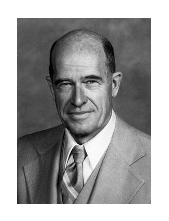
\includegraphics[width=0.9\linewidth]{WalterEvans.eps} 
    \caption*{\textbf{Walter Richard Evans}, (1920-1999),ingénieur, 
              automaticien américain. Il développa la méthode graphique, 
              qui porte son nom, permettant d'étudier les pôles des 
              systèmes asservis.}
\end{marginfigure}
%-------------------------------------------------------------------------------
pour l'étude des systèmes asservis.
%%%%%%%%%%%%%%%%%%%%%%%%%%%%%%%%%%%%%%%%%%%%%%%%%%%%%%%%%%%%%%%%%%%%%%%%%%%%%%%%
\paragraph{Exemple de carte de pôles et zéros d'une fonction de transfert}
%%%%%%%%%%%%%%%%%%%%%%%%%%%%%%%%%%%%%%%%%%%%%%%%%%%%%%%%%%%%%%%%%%%%%%%%%%%%%%%%
Soit $H(p)$ une fonction de transfert telle que,
%-------------------------------------------------------------------------------
\begin{align}
    H(p)=\dfrac{p-1}{p^2+2p+2}\label{eq-ft_carte}
\end{align}
%-------------------------------------------------------------------------------
Cette fonction de transfert possède un zéro réel ($z_1=1$) et deux 
pôles complexes conjugués ($p_{1,2}=-1\pm j$).
La forme factorisée de $H(p)$ est donc
%-------------------------------------------------------------------------------
\begin{align} 
    H(p)=\dfrac{p-1}{(p+1+j)(p+1-j)}
\end{align}
%-------------------------------------------------------------------------------
La~\cref{fig-carte} présente la carte des pôles de cette fonction de transfert.
%-------------------------------------------------------------------------------
\begin{figure}[!h]
    \center
    \tikzsetnextfilename{carte-chap_slci-ext}
    \input{tikz/carte-chap_slci.tex}
    \caption{Exemple d'une carte de pôles et zéros associés à la 
             fonction de transfert~\Cref{eq-ft_carte}\label{fig-carte}}
\end{figure}
%-------------------------------------------------------------------------------
%%%%%%%%%%%%%%%%%%%%%%%%%%%%%%%%%%%%%%%%%%%%%%%%%%%%%%%%%%%%%%%%%%%%%%%%%%%%%%%%
%%%%%%%%%%%%%%%%%%%%%%%%%%%%%%%%%%%%%%%%%%%%%%%%%%%%%%%%%%%%%%%%%%%%%%%%%%%%%%%%
%\subsection{Notion de pôles dominants}
%%%%%%%%%%%%%%%%%%%%%%%%%%%%%%%%%%%%%%%%%%%%%%%%%%%%%%%%%%%%%%%%%%%%%%%%%%%%%%%%
%%%%%%%%%%%%%%%%%%%%%%%%%%%%%%%%%%%%%%%%%%%%%%%%%%%%%%%%%%%%%%%%%%%%%%%%%%%%%%%%
%Soient $p_1,\ldots,p_n$ les pôles d'un système stable\footnote{À partir 
%des résultats obtenus dans ce chapitre il est déjà clair que la stabilité
%d'un système dépend également des pôles de sa fonction de transfert}.
%Le pôle $p_i$ est dit dominant si la valeur absolue
%de sa partie réelle est largement plus petite que celle de tout autre pôles 
%du système\footnote{Dans la pratique un rapport de 5 est 
%suffisant pour considérer une domination d'un pôle sur les autres}
%-------------------------------------------------------------------------------
%\begin{bequation}[ams align]
%	\big|\Re{p_i}\big| \ll \big|\Re{p_j}\big|\;\; \forall j\neq i
%\end{bequation}
%-------------------------------------------------------------------------------
%Pour observer l'influence d'un pôle dominant sur 
%la réponse temporelle d'un système linéaire, nous
%nous allons l'illustrer par l'étude d'une fonction 
%de transfert du second ordre en régime apériodique.
%Une telle fonction de transfert est équivalente à deux
%systèmes du premier ordre en série.

%Prenons l'exemple de la fonction de transfert définie par  
%\[
%       H(p)=\dfrac{5}{(p+1)(5p+1)}
%\]
%et de décomposition en éléments simples telle que :
%\[
%       H(p)=\dfrac{A}{p+1}+\dfrac{B}{5p+1}
%\]
%Par identification on peut écrire $H(p)$ en fonction de
%deux fonctions de transferts $H_1(p)$ et $H_2(p)$ tel que :
%-------------------------------------------------------------------------------
%\begin{align*}
%	H(p)&=H_1(p)-H_2(p)\\
%	H_1(p)&=\dfrac{6.25}{5p+1}\\
%	H_2(p)&=\dfrac{1.25}{p+1}
%\end{align*}
%-------------------------------------------------------------------------------
%Par définition, le pôle dominant est donné par $H_1(p)$.
%Pour observer son effet traçons les réponses indicielles 
%de ces trois fonctions de transfert.
%-------------------------------------------------------------------------------
%\begin{figure}[!h]
%    \centering
%    \tikzsetnextfilename{pole_dominant-chap_slci-ext}
%    \input{tikz/pole_dominant-chap_slci.tex}
%    \caption{}
%\end{figure}
%-------------------------------------------------------------------------------
%-------------------------------------------------------------------------------
%Exercice
%La même approche appliquée pour la fonction cosinus, nous donne :
%-------------------------------------------------------------------------------
%\begin{bequation}[ams align]
%    \laplace{\cos{\omega t}\cdot u(t)}=\dfrac{p}{p^2+\omega^2}
%\end{bequation}
%-------------------------------------------------------------------------------
%Exercice
%%%%%%%%%%%%%%%%%%%%%%%%%%%%%%%%%%%%%%%%%%%%%%%%%%%%%%%%%%%%%%%%%%%%%%%%%%%%%%%%
%\paragraph{Transformée d'une sinuso\"ide amortie}
%%%%%%%%%%%%%%%%%%%%%%%%%%%%%%%%%%%%%%%%%%%%%%%%%%%%%%%%%%%%%%%%%%%%%%%%%%%%%%%%
%La transformée de Laplace d'un signal sinuso\"idal amortie s'écrit :
%-------------------------------------------------------------------------------
%\begin{align*}
%\laplace{e^{-at}\sin{\omega t}\cdot u(t)}&=\int_{0}^{+\infty}e^{-pt}e^{-at}
%\dfrac{e^{\jw t}-e^{-\jw t}}{2j}\dd{t}\\
%&=\dfrac{1}{2j}\int_{0}^{+\infty}e^{-((p+a)-\jw)t}\dd{t} - 
%\dfrac{1}{2j}\int_{0}^{+\infty}e^{-((p+a)+\jw)t}\dd{t} \\
%&=\dfrac{1}{2j}\left( \dfrac{1}{(p+a)-\jw}-\dfrac{1}{(p+a)+\jw}\right)\\
%&=\dfrac{\omega}{(p+a)^2+\omega^2}
%\end{align*}
%-------------------------------------------------------------------------------
%ou encore
%-------------------------------------------------------------------------------
%\begin{bequation}[ams align]
%    \laplace{e^{-at}\sin{\omega t}\cdot u(t)}=\dfrac{\omega}{(p+a)^2+\omega^2}
%\end{bequation}
%-------------------------------------------------------------------------------
%Remarquons que pour cette transformée, nous aurions pu faire usage
%de la propriété du théorème de l'amortissement (c.f propriétés du paragraphe 
%précédent).
\newpage
%%%%%%%%%%%%%%%%%%%%%%%%%%%%%%%%%%%%%%%%%%%%%%%%%%%%%%%%%%%%%%%%%%%%%%%%%%%%%%%%
%%%%%%%%%%%%%%%%%%%%%%%%%%%%%%%%%%%%%%%%%%%%%%%%%%%%%%%%%%%%%%%%%%%%%%%%%%%%%%%%
%%%%%%%%%%%%%%%%%%%%%%%%%%%%%%%%%%%%%%%%%%%%%%%%%%%%%%%%%%%%%%%%%%%%%%%%%%%%%%%%
\section{Exercices du chapitre}
%%%%%%%%%%%%%%%%%%%%%%%%%%%%%%%%%%%%%%%%%%%%%%%%%%%%%%%%%%%%%%%%%%%%%%%%%%%%%%%%
%%%%%%%%%%%%%%%%%%%%%%%%%%%%%%%%%%%%%%%%%%%%%%%%%%%%%%%%%%%%%%%%%%%%%%%%%%%%%%%%
%%%%%%%%%%%%%%%%%%%%%%%%%%%%%%%%%%%%%%%%%%%%%%%%%%%%%%%%%%%%%%%%%%%%%%%%%%%%%%%%
\small
%{\tikzset{external/export=false} 
\makeatletter
\newcount\my@repeat@count
\newcommand{\myrepeat}[2]{%
    \begingroup
    \my@repeat@count=\z@
    \@whilenum\my@repeat@count<#1\do{#2\advance\my@repeat@count\@ne}%
    \endgroup
}
\makeatother
\newcommand{\mystar}{{\color{col1}\fontfamily{lmr}\selectfont$\star$}}
\newcommand{\facile}{\marginpar{\myrepeat{1}{\mystar}}}
\newcommand{\moyen}{\marginpar{\myrepeat{2}{\mystar}}}
\newcommand{\difficile}{\marginpar{\myrepeat{3}{\mystar}}}
\newcommand{\tresdifficile}{\marginpar{\myrepeat{4}{\mystar}}}
%%%%%%%%%%%%%%%%%%%%%%%%%%%%%%%%%%%%%%%%%%%%%%%%%%%%%%%%%%%%%%%%%%%%%%%%%%%%%%%%
%%%%%%%%%%%%%%%%%%%%%%%%%%%%%%%%%%%%%%%%%%%%%%%%%%%%%%%%%%%%%%%%%%%%%%%%%%%%%%%%
\moyen\exercice{L'impulsion de Dirac approchée}
%%%%%%%%%%%%%%%%%%%%%%%%%%%%%%%%%%%%%%%%%%%%%%%%%%%%%%%%%%%%%%%%%%%%%%%%%%%%%%%%
%%%%%%%%%%%%%%%%%%%%%%%%%%%%%%%%%%%%%%%%%%%%%%%%%%%%%%%%%%%%%%%%%%%%%%%%%%%%%%%%
L'impulsion de Dirac peut être approchée par la fonction porte 
$\delta_a(t)$ définie par le graphe ci-contre.

%%%%%%%%%%%%%%%%%%%%%%%%%%%%%%%%%%%%%%%%%%%%%%%%%%%%%%%%%%%%%%%%%%%%%%%%%%%%%%%%
\question{Décomposer $\delta_a(t)$ à l'aide de fonctions échelons.}
%%%%%%%%%%%%%%%%%%%%%%%%%%%%%%%%%%%%%%%%%%%%%%%%%%%%%%%%%%%%%%%%%%%%%%%%%%%%%%%%
%-------------------------------------------------------------------------------
\begin{marginfigure}
    \centering
    \tikzsetnextfilename{fonction_porte-chap-slci-ext}
    \begin{tikzpicture}[baseline=0]
   \begin{axis}[
        height=4cm,
        width=5cm,
        axis x line=center,
        axis y line=center,
        xmin=-1,
        xmax=5,
        ymin=-0.5,
        ymax=2.0,
        xlabel={$t$},
        ylabel={$\delta_a(t)$},
        xlabel style={below right},
        ylabel style={left},
        yticklabels={$\dfrac{1}{a}$},
        ytick={1},
        y tick label style={anchor=east},
        xticklabels={$a$},
        xtick={2},
        x tick label style={anchor=north},
        ]
        \addplot [very thick,col1,const plot] coordinates 
        {(-1,0.01) (0,0.01) (0,1) (2,1)  (2,0.01) (5,0.01) };
        \end{axis}
\end{tikzpicture}

\end{marginfigure}
%-------------------------------------------------------------------------------

%%%%%%%%%%%%%%%%%%%%%%%%%%%%%%%%%%%%%%%%%%%%%%%%%%%%%%%%%%%%%%%%%%%%%%%%%%%%%%%%
\question{Donner sa transformée de Laplace en fonction du paramètre $a$.}
%%%%%%%%%%%%%%%%%%%%%%%%%%%%%%%%%%%%%%%%%%%%%%%%%%%%%%%%%%%%%%%%%%%%%%%%%%%%%%%%

%%%%%%%%%%%%%%%%%%%%%%%%%%%%%%%%%%%%%%%%%%%%%%%%%%%%%%%%%%%%%%%%%%%%%%%%%%%%%%%%
\question{En considérant la limite $a\rightarrow0$, montrer que la transformée
          de Laplace de $\delta_a(t)$ tend bien vers 1.}
%%%%%%%%%%%%%%%%%%%%%%%%%%%%%%%%%%%%%%%%%%%%%%%%%%%%%%%%%%%%%%%%%%%%%%%%%%%%%%%%

%%%%%%%%%%%%%%%%%%%%%%%%%%%%%%%%%%%%%%%%%%%%%%%%%%%%%%%%%%%%%%%%%%%%%%%%%%%%%%%%
\question{Soit la fonction $g_a(t)$ définie par le graphe ci-contre. 
          Décomposer $g_a(t)$ à l'aide de fonctions échelons et/ou rampes. Donner sa 
          transformée de Laplace.}
%%%%%%%%%%%%%%%%%%%%%%%%%%%%%%%%%%%%%%%%%%%%%%%%%%%%%%%%%%%%%%%%%%%%%%%%%%%%%%%%
%-------------------------------------------------------------------------------
\begin{marginfigure}
    \centering
    \tikzsetnextfilename{fonction_creneau-chap-slci-ext}
    \input{tikz/fonction_creneau-chap-slci.tex}
\end{marginfigure}
%-------------------------------------------------------------------------------

%}
\setcounter{numexos}{0}
\normalsize
\newpage
\restoregeometry
\captionsetup{width=0.9\linewidth,labelfont=bf}
%%%%%%%%%%%%%%%%%%%%%%%%%%%%%%%%%%%%%%%%%%%%%%%%%%%%%%%%%%%%%%%%%%%%%%%%%%%%%%%%
%%%%%%%%%%%%%%%%%%%%%%%%%%%%%%%%%%%%%%%%%%%%%%%%%%%%%%%%%%%%%%%%%%%%%%%%%%%%%%%%
%%%%%%%%%%%%%%%%%%%%%%%%%%%%%%%%%%%%%%%%%%%%%%%%%%%%%%%%%%%%%%%%%%%%%%%%%%%%%%%%
\section{Corrigé des exercices}
%%%%%%%%%%%%%%%%%%%%%%%%%%%%%%%%%%%%%%%%%%%%%%%%%%%%%%%%%%%%%%%%%%%%%%%%%%%%%%%%
%%%%%%%%%%%%%%%%%%%%%%%%%%%%%%%%%%%%%%%%%%%%%%%%%%%%%%%%%%%%%%%%%%%%%%%%%%%%%%%%
%%%%%%%%%%%%%%%%%%%%%%%%%%%%%%%%%%%%%%%%%%%%%%%%%%%%%%%%%%%%%%%%%%%%%%%%%%%%%%%%
\small
%%%%%%%%%%%%%%%%%%%%%%%%%%%%%%%%%%%%%%%%%%%%%%%%%%%%%%%%%%%%%%%%%%%%%%%%%%%%%%%%
%%%%%%%%%%%%%%%%%%%%%%%%%%%%%%%%%%%%%%%%%%%%%%%%%%%%%%%%%%%%%%%%%%%%%%%%%%%%%%%%
\exercice{L'impulsion de Dirac approchée}
%%%%%%%%%%%%%%%%%%%%%%%%%%%%%%%%%%%%%%%%%%%%%%%%%%%%%%%%%%%%%%%%%%%%%%%%%%%%%%%%
%%%%%%%%%%%%%%%%%%%%%%%%%%%%%%%%%%%%%%%%%%%%%%%%%%%%%%%%%%%%%%%%%%%%%%%%%%%%%%%%
%%%%%%%%%%%%%%%%%%%%%%%%%%%%%%%%%%%%%%%%%%%%%%%%%%%%%%%%%%%%%%%%%%%%%%%%%%%%%%%%
\question{}
%%%%%%%%%%%%%%%%%%%%%%%%%%%%%%%%%%%%%%%%%%%%%%%%%%%%%%%%%%%%%%%%%%%%%%%%%%%%%%%%
%-------------------------------------------------------------------------------
\begin{figure}[!h]
    \centering
    \tikzsetnextfilename{fonction_porte_decomposition-chap-slci-ext}
    \input{tikz/fonction_porte_decomposition-chap-slci.tex}
\end{figure}
%-------------------------------------------------------------------------------
La fonction $\delta_a(t)$ est simplement donnée par 
\[
    \color{col1}p_a(t)
    =\color{col4}\dfrac{1}{a}u(t)\color{col3}-\dfrac{1}{a}u(t-a)
    =\normalcolor\dfrac{1}{a}\left(u(t)-u(t-a)\right)
\] 
où $u(t)$ est la fonction échelon unité.

%%%%%%%%%%%%%%%%%%%%%%%%%%%%%%%%%%%%%%%%%%%%%%%%%%%%%%%%%%%%%%%%%%%%%%%%%%%%%%%%
\question{}
%%%%%%%%%%%%%%%%%%%%%%%%%%%%%%%%%%%%%%%%%%%%%%%%%%%%%%%%%%%%%%%%%%%%%%%%%%%%%%%%
On rappel la transformée de Laplace d'une fonction retardée :
\[
    \laplace{f(t-\tau)} = e^{-\tau p}F(p)
\]
La transformée de Laplace de $\delta_a(t)$ est donc donnée par : 
\[
    \Delta_a(p) = \laplace{\delta_a(t)}
                = \dfrac{1}{a}\left(\laplace{u(t)}-\laplace{u(t-a)}\right)
                = \dfrac{1}{ap}(1-e^{-ap})
\]
%%%%%%%%%%%%%%%%%%%%%%%%%%%%%%%%%%%%%%%%%%%%%%%%%%%%%%%%%%%%%%%%%%%%%%%%%%%%%%%%
\question{}
%%%%%%%%%%%%%%%%%%%%%%%%%%%%%%%%%%%%%%%%%%%%%%%%%%%%%%%%%%%%%%%%%%%%%%%%%%%%%%%%
Le développement limité d'ordre 1 de $e^{x}=1+x+o\left(x\right)$ permet de
déterminer la limite pour $a\rightarrow0$ de la transformée de Laplace de 
$\delta_a(t)$. En effet, 
\[
    \lim_{a\to0} \Delta_a(p) = \dfrac{1}{ap}(1-1+ap)=1.
\]
Puisque la transformée de Laplace d'une impulsion de Dirac est égale à 1, on a
bien vérifié que $\lim_{a\to0} \delta_a(p)=\delta(t)$ où $\delta(t)$ est 
l'impulsion de Dirac.

%%%%%%%%%%%%%%%%%%%%%%%%%%%%%%%%%%%%%%%%%%%%%%%%%%%%%%%%%%%%%%%%%%%%%%%%%%%%%%%%
\question{Soit la fonction $g_a(t)$ définie par le graphe ci-contre. 
          Décomposer $g_a(t)$ à l'aide de fonctions échelons et/ou rampes. Donner sa 
          transformée de Laplace.}
%%%%%%%%%%%%%%%%%%%%%%%%%%%%%%%%%%%%%%%%%%%%%%%%%%%%%%%%%%%%%%%%%%%%%%%%%%%%%%%%
%-------------------------------------------------------------------------------
\begin{marginfigure}
    \centering
    \tikzsetnextfilename{fonction_creneau-chap-slci-ext}
    \begin{tikzpicture}[baseline=0]
   \begin{axis}[
   height=4cm,
   width=5cm,
      axis x line=center,
        axis y line=center,
        xmin=-1,
        xmax=5,
        ymin=-1.5,
        ymax=2.0,
        xlabel={$t$},
        ylabel={$g_a(t)$},
        xlabel style={below right},
        ylabel style={left},
        yticklabels={$\dfrac{1}{a}$},
        ytick={1},
        y tick label style={left},
        xticklabels={$\tau+a$,$\tau+2a$},
        xtick={2,4},
        x tick label style={below},
        ]
        \addplot [very thick,col1,domain=-1:0, samples=50]{0.01};
        \addplot [very thick,col1,domain=0:2, samples=50]{0.5*x};
        \addplot [very thick,col1,domain=2:4, samples=50]{-0.5*x+2};
        \addplot [very thick,col1,domain=4:5, samples=50]{0.01};
        \end{axis}
\end{tikzpicture}

\end{marginfigure}
%-------------------------------------------------------------------------------

\[
    g_a(t)=\dfrac{1}{a(\tau+a)}r(t)-\dfrac{2}{a(\tau+a)}r(t-(\tau+a))+\dfrac{1}{a(\tau+a)}r(t-(\tau+2a))
\]

\[
    g_a(t)=\dfrac{t}{a(\tau+a)}u(t)
\]

\[
    -\dfrac{t}{a(\tau+a)}-\dfrac{1}{\tau+a}-\dfrac{1}{a}=\dfrac{t}{a(\tau+a)}+f_2(t)
\]

\[
    -\dfrac{2t-(\tau+2a)}{a(\tau+a)}=f_2(t)
\]

\[
    g_a(t)=\dfrac{t}{a(\tau+a)}u(t)-\dfrac{2t-(\tau+2a)}{a(\tau+a)}u(t-(\tau+a))
\]

\[
    f_3(t)=\dfrac{t-(\tau+2a)}{a(\tau+a)}
\]

\[
    g_a(t)=\dfrac{t}{a(\tau+a)}u(t)-\dfrac{2t-(\tau+2a)}{a(\tau+a)}u(t-(\tau+a))+\dfrac{t-(\tau+2a)}{a(\tau+a)}u(t-(\tau+2a))
\]

\[
    g_a(t)=\dfrac{1}{a(\tau+a)}\left(t-(2t-(\tau+2a))u(t-(\tau+a))+(t-(\tau+2a))u(t-(\tau+2a))\right)
\]

\footnotesize
\[
    \laplace{g_a(t)}=\dfrac{1}{a(\tau+a)}\left(   \dfrac{1}{p^2}-\dfrac{2e^{-(\tau+a)p}}{p^2}+\dfrac{(\tau+2a)e^{-(\tau+a)p}}{p}
                                                + \dfrac{e^{-(\tau+2a)p}}{p^2} - \dfrac{(\tau+2a)e^{-(\tau+2a)p}}{p} \right)
\]
\[
     \laplace{g_a(t)}=\dfrac{1}{a(\tau+a)}\left( \dfrac{1}{p^2}\left(1-2e^{-(\tau+a)p}+e^{-(\tau+2a)p}\right) 
                                           + \dfrac{(\tau+2a)}{p}\left(e^{-(\tau+a)p}-e^{-(\tau+2a)p} \right) \right)
\]


\[
    e^{-(\tau+a)p}=e^{-\tau p}e^{-ap}=e^{-\tau p}\left(1-ap+\dfrac{(ap)^2}{2}\right)
\]

\[
    e^{-(\tau+2a)p}=e^{-\tau p}e^{-2ap}=e^{-\tau p}\left(1-2ap+2(ap)^2\right)
\]

\[
    1-2e^{-(\tau+a)p}+e^{-(\tau+2a)p}=1-e^{-\tau p}\left(1-ap+\dfrac{(ap)^2}{2}\right)+e^{-\tau p}\left(1-2ap+2(ap)^2\right)
\]

\[
    1-2e^{-(\tau+a)p}+e^{-(\tau+2a)p}=1-ape^{-\tau p}+\dfrac{3}{2}(ap)^2e^{-\tau p}
\]

\[
    e^{-(\tau+a)p}=e^{-\tau p}e^{-ap}=e^{-\tau p}\left(1-ap\right)
\]

\[
    e^{-(\tau+2a)p}=e^{-\tau p}e^{-ap}=e^{-\tau p}\left(1-2ap\right)
\]

\[
    e^{-(\tau+a)p}-e^{-(\tau+2a)p}=ape^{-\tau p}
\]

\[
    \laplace{g_a(t)}=\dfrac{1}{a(\tau+a)}\left(\right)
\]


\[
    g_a(t)=\dfrac{t}{a(\tau+a)}\left(u(t)-u(t-(\tau+a))\right) - \left(\dfrac{t-(\tau+2a)}{a(\tau+a)}\right)\left(u(t-(\tau+a))-u(t-(\tau+2a))\right)
\]

\[
    \laplace{g_a(t)}=\dfrac{1}{a(\tau+a)p^2}\left(1-e^{-(\tau+a)p}\right) - \dfrac{1}{a(\tau+a)}\left(\dfrac{1}{p^2}-\dfrac{(\tau+2a)}{p}\right)\left(e^{-(\tau+a)p}-e^{-(\tau+2a)p}\right)
\]

\normalsize
\restoregeometry
\captionsetup{width=0.9\linewidth,labelfont=bf}
%%%%%%%%%%%%%%%%%%%%%%%%%%%%%%%%%%%%%%%%%%%%%%%%%%%%%%%%%%%%%%%%%%%%%%%%%%%%%%%%
%%%%%%%%%%%%%%%%%%%%%%%%%%%%%%%%%%%%%%%%%%%%%%%%%%%%%%%%%%%%%%%%%%%%%%%%%%%%%%%%
%%%%%%%%%%%%%%%%%%%%%%%%%%%%%%%%%%%%%%%%%%%%%%%%%%%%%%%%%%%%%%%%%%%%%%%%%%%%%%%%
%%%%%%%%%%%%%%%%%%%%%%%%%%%%%%%%%%%%%%%%%%%%%%%%%%%%%%%%%%%%%%%%%%%%%%%%%%%%%%%%
%chap_slci.tex
